\chapter{算法与实现}\label{chap:algo}

\begin{flushleft}  %% 左对其(临时添加)
\setlength{\parindent}{2em} %% 首行缩进(临时添加)

\qquad  

过去十年来高性能计算经历了从十万亿次到百万亿次再到千万亿次的突破,高性能算法设计与优化面临着利用并行性(并行墙)和开发局部性(内存墙)的难题,增加并行度和更深的内存层次可持续提升高性能计算机系统性能,同时对高性能算法设计带来了新挑战,尤其是多核、众核引入的多层次大规模并行(并行墙)并导致内存到计算部件供数不足的问题(内存墙)愈加恶化,因此,如何缓解扩展并行而恶化的访存瓶颈成为高性能计算算法与实现的核心问题,需要通过并行算法模型和实现优化上不断创新。
本章旨在论述数据流思想在解决上述高性能计算关键问题的研究,基于数据流模型,提出适应众核体系结构算法设计和优化的“渗透执行”的算法设计模型,并通过科学计算、组合优化和大数据分析应用的核心算法的实践,展示数据流技术在高性能计算算法设计和优化方面的优势。

\section{导言和背景}
\subsection{导言}
本章介绍基于数据流思想的高性能算法设计和优化技术,其基本动机是众核体系结构发展驱动新的高性能算法模型的提出,渗透模型是其中代表之一。下面几节描述渗透模型及其在典型高性能计算算法中的应用。

关于渗透算法模型的介绍,\ref{sec:percolation}节的逻辑结构是先解释什么是渗透,然后描述如何渗透,包括其基本原理~\ref{sec:percolation_what}、关键技术~\ref{sec:percolation_how}和实现方法~\ref{sec:percolation_method}。

接下来三节展示渗透模型在三个典型算法中的应用,依次是组合优化问题动态规划算法~\ref{sec:PM_dp}、大数据分析图计算~\ref{sec:PM_graph}和科学计算问题稠密矩阵乘~\ref{sec:PM_mm},分别代表了强数据依赖关系、极低数据局部性和规则计算三类问题。从一定程度上验证了基于数据流的渗透模型是一种通用型的高性能算法设计和优化方法。

\subsection{背景}

在高性能计算机系统性能到达P级以后,尤其是以众核为主流的处理器结构的出现,并行性大幅增加,数据通路能力提升缓慢,导致了严重的数据访问(访存、通信)瓶颈,P级应用呈现出数据密集、算法计算访存比低且模式多样的新特点,一味提高硬件系统的峰值性能对实际应用的性能提升帮助不大,算法优化研究成为挖掘高性能计算机实际计算能力的关键,特别是需要适应不同计算访存比的算法优化方法,以提高80\%以上实际应用在“通用型”高性能计算机上的性能。

从高性能算法设计和性能优化的历史角度看,经历了单核、多核和众核三个阶段。在单核处理器结构,算法设计核优化以挖掘程序中的局部性(时间局部性和空间局部性)为核心,重点研究数据布局和存取策略以适应基于cache内存层次的体系结构。到了多核和多处理器时代,并行性的有效挖掘和利用成为关键,提高算法的扩展性是优化的主要目标。众核处理器由于提供了大量的片内并行,局部性和并行性必须是同时考虑的双重目标。纵观已有的执行模型,数据流具有统一局部性和并行性的天然优势。

\begin{figure}[!htbp]
	\centering
	%trim option's parameter order: left bottom right top
	\includegraphics[clip, scale=0.4]{Img/Chap_Algorithm/background}
	\bicaption{性能优化决定了实际峰值。}{Performance optimizations.}
	\label{fig:background}
\end{figure}

\section{基于数据流的高性能算法模型}\label{sec:percolation}

为了缓解日益加剧的“存储墙”(Memory Wall)对高性能算法在多核和众核体系结构上执行性能(计算效率和并行扩展性)的影响,谭光明等~\citep{TanThesis,TanTPDS09}在2008年提出了基于数据流的渗透算法设计模型,以适应高性能计算机系统的计算引擎以众核为主流的趋势。本质上讲,基于数据流的渗透模型(Percolation Model)利用众核体系结构存在的并行为计算操作提供数据访问的局部性,是一种高度融合并行性和局部性的延迟容忍的性能优化技术。本小节从基本原理、关键技术和算法设计方法三个方面介绍渗透模型。

\subsection{渗透模型的基本原理}\label{sec:percolation_what}
从算法设计和优化的角度看,两个主要因素是并行性和局部性。传统的并行算法设计模型中,并行性和局部性是割裂开独立考虑,并行任务的划分和映射仅仅最多考虑到静态数据的亲和性。在数据流执行模型中,并行性和局部性通过以数据为中心而天然统一存在与程序的执行过程中,数据流中actor的firing隐含了所依赖操作并行性和数据局部性的统一,以数据驱动计算的机制执行程序流。基于并行性和局部性统一的数据流思想,面向众核体系结构的渗透模型利用众核天然的并行,实现把数据“推”送到被需要的地方,达到数据驱动计算的效果。

在基于非数据流的执行模型中,每个处理器核在其计算操作执行需要相关数据操作的时刻才发起读取数据的请求,自己从内存中“拉”数据。基于数据流的执行模型,计算操作所依赖的数据通过某种机制在启动计算之前已经被“推”送过来。在集成了大规模片上处理器核的众核架构中,这种“推”送机制可由一些空闲的核完成,因此,在整个程序运行过程中,数据在负责计算操作的处理器核无参与的情况下在不同存储层级中移动,称之为“渗透”(Percolation)。这样在理想情况下,程序的运行过程开销只有有效的计算操作时间。

\begin{figure}[!htbp]
	\centering
	%trim option's parameter order: left bottom right top
	\includegraphics[clip, scale=0.6]{Img/Chap_Algorithm/percolation_what}
	\bicaption{渗透模型的基本原理}{The principle of percolation model.}
	\label{fig:percolation_what}
\end{figure}

如图\ref{fig:percolation_what}所示一个抽象的众核体系结构,众核处理器有$n$个核心,两级内存结构:缓存和内存。“内存墙”瓶颈指的就是通过内存总线访问内存里面的数据,随着处理器中计算核的处理能力增强,性能瓶颈愈加突出。在基于数据流的渗透模型中,在某一个运行时刻,核0主动把核2计算操作所依赖的数据提前从内存移动到缓存中,在核2需要的时候推送给它,这样核2直接从缓存中读取数据,由于在体系结构实现中,缓存通路高带宽和低延迟,从而缓解了“内存墙”的性能瓶颈。

\subsection{渗透模型的关键技术}\label{sec:percolation_how}

渗透模型是为众核体系结构性能优化构建的,多线程是众核体系结构上主流并行机制。在常规的多线程执行中,一旦一个线程需要的数据和控制依赖关系在逻辑上得到满足,该线程就开始启动计算操作。这种弱执行模型对具有高度局部性的规则计算模式能够获得高的性能,然而非规则计算不存在明显的局部性甚至无局部性,弱执行模型不能利用局部性优化提高性能。为了获得非规则计算中的局部性,渗透模型要求线程的执行必须同时满足两个条件:1)数据和控制依赖关系;2)局部性依赖关系(locality dependence)。后者强制线程执行前需要的数据必须位于其局部存储空间中,即渗透模型的关键:即时局部性(just-in-time locality)。

\begin{figure}[!htbp]
	\centering
	%trim option's parameter order: left bottom right top
	\includegraphics[clip, scale=0.6]{Img/Chap_Algorithm/percolation_how}
	\bicaption{渗透模型的关键技术:即时局部性}{Just-in-time locality.}
	\label{fig:percolation_how}
\end{figure}

在多线程编程模型中,一个线程的工作为一个任务,这样,程序表示成有向无环任务图,图中的顶点表示任务,边代表了两个任务间的依赖关系,如图\ref{fig:percolation_how}。一个顶点$s$(任务/线程)被激活的条件是其前驱操作完成,而且该任务的数据和控制依赖关系得到满足。一个任务仅满足控制和数据依赖关系,称之处于逻辑活跃。在渗透模型中,如果所依赖的数据没有位于待执行任务的局部存储空间,逻辑上活跃的任务不能被调度执行。只有当它的局部性依赖关系得到满足,该逻辑上活跃的任务启动计算。基于众核体系结构的渗透模型中,这种局部性依赖关系由空闲核运行时创建。

为了创建即时局部性,渗透模型要求对算法中的计算和访存操作分离。通过解耦计算和访存,并行算法可以:1)通过访存任务和计算任务之间的多级流水隐藏存储访问的开销;2)组织和分配不同的访存任务来适应存储层次结构中的不同访问延迟,如非连续地址到连续存储区域的变换。在多线程环境中,由某个独立的线程单元称为渗透线程负责存储层次之间的数据移动。尽管渗透在一定程度上与预期机制由共同之处,但又不同于常规的预取,主要体现在下面两个特征:

\begin{itemize}	
	\item {\bf 按需取数}:只有当某个线程需要访问数据时,该数据才出现在片内存储中。如果数据已经在片内存储中,
	该数据马上就会被使用;一段数据的地址即使和刚刚被访问的高延迟存储中的数据的地址连续,如果不需要马上被使用,也不会出现在低延迟存储中。

	\item {\bf 数据变换}:渗透要求在存储层次间聚合/分散数据和对数据组织进行变换,高延迟存储中的离散的存储访问可以在渗透过程中聚合成连续的低延迟存储访问,从而获得局部存储访问的局部性。
\end{itemize}

\subsection{渗透模型的实现方法}\label{sec:percolation_method}

事实上,体系结构支持用户级的计算和访存操作分离已经成为高性能计算机系统的趋势。基于消息传递的并行计算机系统支持零拷贝的RDMA机制(事实上目前
所有的高性能网络设备如Infiniband等都有该特征,并且有相应软件环境),消息传递操作看成访问远程机器的内存。多核结构中通过多线程(如IBM Cyclops64、GPU)或者DMA(如IBM Cell、申威众核)的方式支持异步的存储操作。无论是分布式存储还是共享存储结构,在本文提出抽象机器模型中,
有如下假设:
\begin{itemize}
	\item {\bf 二级存储模型:}所有的处理单元能够直接访问任何的存储空间。相对于每个处理单元,存储空间根据访问延迟的差异划分成延迟相对较低的in-core memory (ICM)和较高的out-of-core memory(OCM),而ICM又可以进一步在多个处理器之间划分成若干in-core local memory(ICLM)。
	\item {\bf 强执行模型:}只有当计算所需要的数据已经在ICM/ICLM时,计算才开始。而且只有当计算的线城需要某数据时,该数据才出现在ICM/ICLM中。
	\item {\bf 细粒度并行:}计算和访问OCM操作能够同时进行
\end{itemize}

通常而言,显式存储层次结构的片内存储比片外存储尺寸小很多,但提供更高的带宽和更低的延迟。目前多核体系结构提供的存储访问延迟容
忍技术主要是多线程和DMA异步传输。如果在两个存储访问之间有足够的计算,则存储访问延迟的问题不会太突出。本章第\ref{sec:PM_graph}介绍的图遍历算法只有少量的计算,
当所有的线程同时访问片外存储时,其延迟和带宽成为性能瓶颈。

在分布式存储体系结构中,节点内部的内存映射为ICM,远程节点的存储映射为OCM;共享存储多核体系结构如IBM
Cyclops64系统中,一个芯片上的SPM和片上SRAM映射为ICM,
SPM可以划分为ICLM,片外DRAM映射为OCM。在基于DMA异步传输的体系结构中,延迟隐藏策略自然地通过DMA实现;多线程体系结构中,需要对线程进行划分,
即分离出一部分线程作为渗透或者{\it helper}线程,这些{\it
	helper}线程负责OCM的访问。在该渗透模型中,通信被抽象为访存操作。

渗透模型强调利用多级并行实现强的执行模型:粗粒度并行用于满足数据和控制依赖关系,细粒度并行获得局部性条件。图~\ref{fig:BasePerc}演示了基本的渗透过程。
{\tiny
	\begin{figure*}[!htbp]
		\begin{center}
			\begin{tabular}{|l|}
				\hline
				\begin{minipage}[t]{4in}
					%{\small
					\begin{tabbing}
						\hspace{.3in} \= {\scshape Percolation Pipelining}\\
						\> XX. \= \kill
						\>  1. \> \b while \= the set of not enabled memory tasks is not empty;\\
						\>       \>\> //stage 1 \\
						\>  2. \> \> A memory tasks $fm(\;)$ becomes enabled;\\
						\>  3. \> \> Data is transformed in off-chip memory;\\
						\>  4. \> \> The transformed data percolates inward to on-chip memory;\\
						\>       \>\> //stage 2 \\
						\>  5. \> \> The code of computation task $fc(\;)$ meeting locality requirement \\
						\>       \>\> percolates inward to on-chip memory;\\
						\>  6. \> \> $fc(\;)$ is enabled;\\
						\>  7. \> \> $fc(\;)$ is retired from on-chip memory;\\
						\>       \>\> //stage 3 \\
						\>  8. \> \> Results are arranged in larger blocks (and transformed)\\
						\>       \> \>  in on-chip memory;\\
						\>  9. \> \> Results are percolated outward to off-chip memory;\\
						\> 10. \> \> Transformations are performed in the outward percolated\\
						\>       \> \>         data in off-chip memory\\
					\end{tabbing}
					%}
				\end{minipage} \\ \hline
			\end{tabular}
			\bicaption{渗透模型流水算法的基本框架}{basic pipelining process (3 stages) of percolation}
			\label{fig:BasePerc}
		\end{center}
	\end{figure*}
}

一个处理单元的执行遵循三个操作状态:LOADLT、STORELT和EXECLT,这三个操作可能同时出现在一个处理单元上,三个操作的定义见表~\ref{tab:notation}。针对异步传输和多线程的差异,
三种操作在这两种体系结构上的调度也存在一定的不同,图\ref{fig:percolation_method}三种操作的并行流水执行模型。渗透模型中,在一个时间步中,
LOADLT/STORELT/EXECLT三种操作状态能够同时出现,为了保证程序的正确执行,该执行模型需要遵循以下执行规则和调度:在执行时间步$t$,计算需要的数据
在时间步$t-1$已经被传输到执行计算的处理单元的ICM/ICLM,其计算结果要到时间步$t+1$时才在必要时传输到OCM中。这种调度策略保证了LOADLT/STORELT/EXECLT
之间没有任何依赖关系,从而可以并行地执行(通过不同的线程单元或者处理单元/DMA设备)。
\begin{table}[!htbp]
	\bicaption{渗透模型流水线中的符号}{Notation convention in percolation pipelining}
	\begin{center}
		\begin{tabular}{|c|c|}
			\hline LOADLT & operations for transferring data from {\em OCM} to {\em ICM}\\\hline
			STORELT & operations for transferring data from {\em ICM} to {\em OCM}\\\hline
			EXECLT & operating data only in {\em ICM}\\\hline
		\end{tabular}
	\end{center}
	\label{tab:notation}
\end{table}

渗透模型强调并行算法设计需要考虑如何获得算法中的计算和访存(通信)之间重叠,同时,由于不同存储空间的访问延迟的差异,并行算法要减少高延迟存储空间的
访问操作,从而,设计渗透模型并行算法需要同时考虑以下两个方面:
\begin{description}
	\item[细粒度并行:]粗粒度并行算法通常掩盖了程序计算行为的细节,特别是把多个计算和访问OCM步骤合并到一个时间步以求算法的简便。设计延迟容忍并行算法要求对算法
	进行更细粒度的划分,挖掘更多的并行步骤,以获得计算和访问OCM的重叠。
	\item[局部性:]尽管访问OCM的开销能够期望通过和计算重叠来隐藏,但毕竟有启动开销和消耗额外的资源(如{\it
		helper}线程)。并行算法设计需要尽量减少访问OCM的操作,增加对ICM中的数据的重用,即提高算法的局部性。
\end{description}
\begin{figure}[htbp]
	\centering
	% Requires \usepackage{graphicx}
	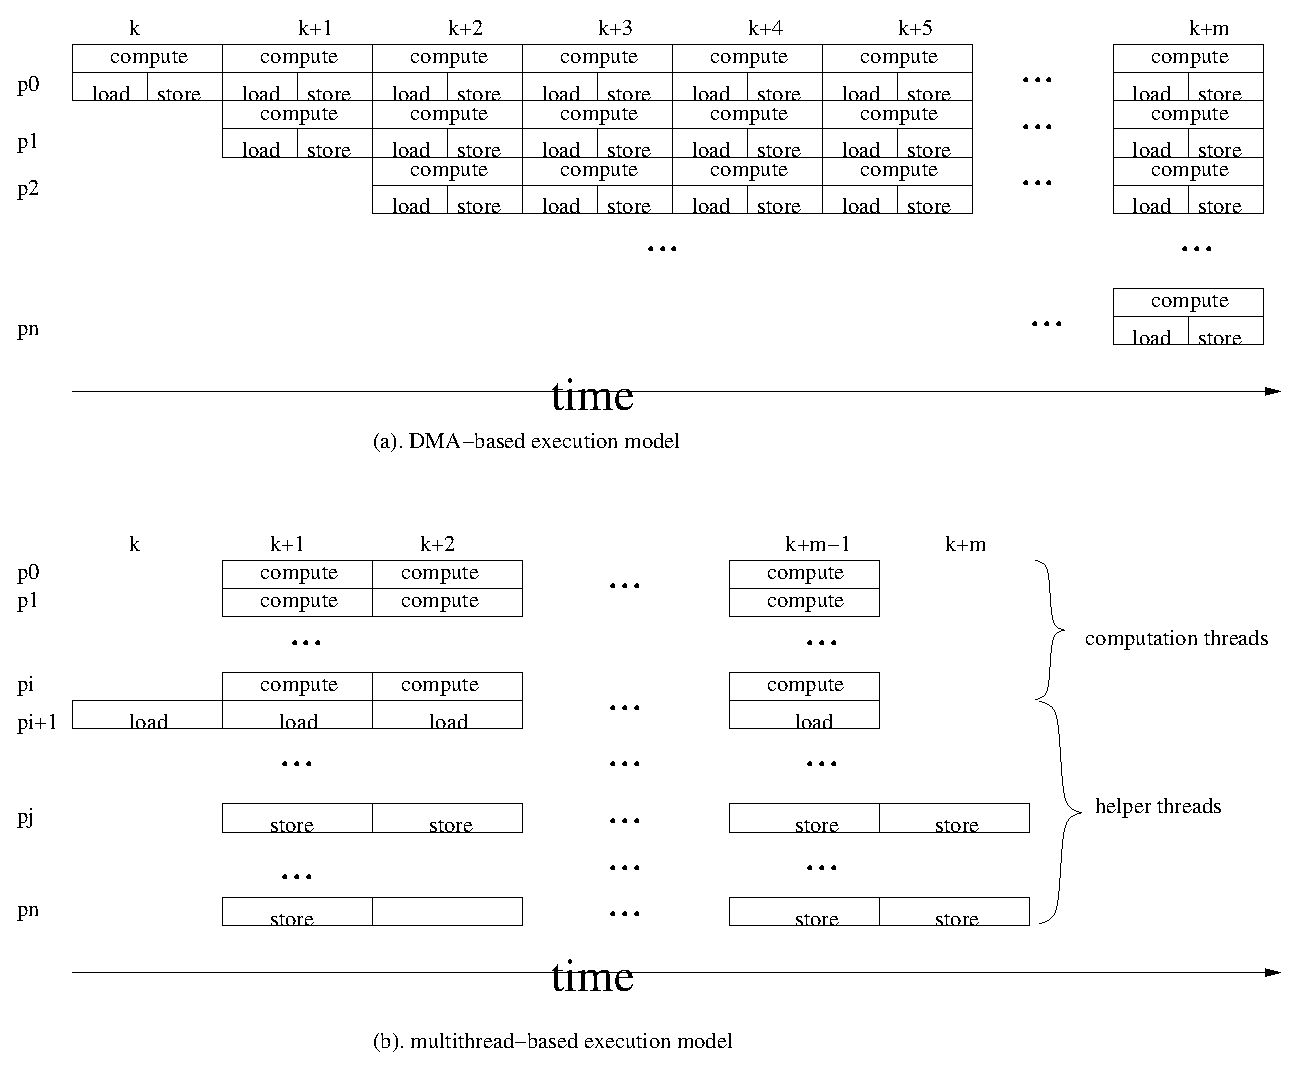
\includegraphics[scale=0.8]{Img/Chap_Algorithm/tolerance_model}\\
	\bicaption{(a). 异步传输的渗透执行模型;(b). 多线程渗透执行模型}{(a). Asynchronous  based percolation; (b). Multithreading based percolation}\label{fig:percolation_method}
	\vspace{-0.5cm}
\end{figure}


\section{组合优化-高性能动态规划算法}\label{sec:PM_dp}

本节介绍对经典组合优化求解算法动态规划的基于渗透模型的并行算法设计和优化。首先给出动态规划算法的基本介绍和重点研究的一类动态规划算法。然后,基于渗透模型的流水线算法实现框架,描述并行动态规划算法。进一步,基于渗透模型的内存层次结构模型,证明了并行算法的最有访存复杂性。最后,在IBM Cyclops64众核处理器结构上进行了实验分析。

\subsection{动态规划算法介绍}
动态规划是求解离散优化问题的一种通用技术,广泛应用于调度问题、仓库管理、自动控制、VLSI设计、交通运输和生物信息学中\citep{dp-book,parallelcomputing-book},其基本思想是将优化问题表达为一
系列的决策过程(求最大或者最小),即形式上表现为一
个决策过程的递归关系式\citep{dp-principle}。设问题{\it r}分解成{\it t}个子问题:$x_{1}, x_{2}, ..., x_{t}$,问题{\it
	r}的解$f(r)$可以表示为:
\begin{equation}\label{op_eq}
r=g(f(x_{1}), f(x_{2}), ..., f(x_{t})
\end{equation}
其中{\it
	g}称为组合函数,它依赖于问题本来的性质。对于优化问题,$g$常常为取最大值或最小值。当$g$取最大值或最小值时,把此方法
称为动态规划法。

求解动态规划的过程通常是填充动态规划矩阵,矩阵中的每一项对应一个子问题,它们的依赖关系根据问题的分解和组合规则确定:如果一
个问题$P$分解成子问题$P_{1}, P_{2}, ..., P_{k}$,问题$P$对应的项的解依赖于$P_{1}, P_{2}, ...,
P_{k}$对应的项的解。动态规划中的子问题之间的依赖关系可用一个有向图$G(V, E)$来表示,图$G$中的一个结点$v_{i}$表示一个子问题,结点$v_{i}$
到
$v_{j}$的边$e_{i,j}$表示结点$v_{i}$表示的子问题的解用于计算$v_{j}$代表的子问题的解。如果有向图无环,图中的结点可以组织成
多级形式,使得第$i$级$level_{i}$的结点的解依赖于其前面一个或者多个级上结点的解。如果任意一级$level_{i}$上的问题的解仅依
赖于$level_{i+1}$上的子问题的解,称之为连续(Serial)动态规划方程,否则如果依赖前面多级子问题的解,称之为非连续的(Nonserial)。
考虑递归方程式,如果一个优化方程中只有一个递归项,称之为一维(Monadic)动态规划方程;如果有多个递归项
,则称 为多维(Polyadic)动态规划方程。基于上述的分类规则,动态规划方程分为连续一维、连续多维、非连续一维和非连续多维
四种形式\citep{parallelcomputing-book}。

本书关注最复杂的一种动态规划即非连续多维动态规划算法,经典的应用有随机上下文无关文法分析\citep{cyk-algo,cyk-algo-1,cyk-algo-2}和矩阵连乘\citep{algorithms-book,matrix-chain}问题,作为计算生物学中重要的问题之一的RNA二级结构预测\citep{rna-pred-bmb,rna-dp,rna-science}也以非连续动态规划算法为核心。为了简化问题以集中分析非连续多维动态规划算法的计算依赖关系,本文使用一种抽象的动态关系方程作为优化目标:
\begin{equation}\label{eq:abstract_dp}
m[i,j] = \left\{ \begin{array}{ll} min_{i \le k < j} \{m[i,j], m[i,k]+m[k+1,j]\} & \textrm{$0 \le i < j < n$}
\\
a(i) & \textrm{$i=j$}
\end{array} \right.
\end{equation}
\begin{figure}[!htbp]
	\begin{center}
		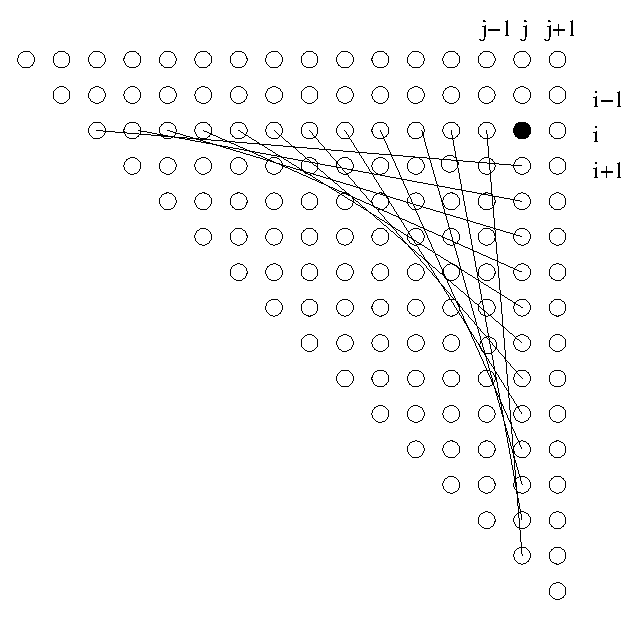
\includegraphics[scale=0.8]{Img/Chap_Algorithm/dp_dependence}
		\caption{非连续多维动态规划算法中的计算依赖关系}\label{fig:dp_dependence}
	\end{center}
\end{figure}

显然,该抽象动态规划方程没有改变非连续多维的计算依赖关系。算法需要计算一个上三角形的动态规划矩阵表,图~\ref{fig:dp_dependence}显示了计算过程中数据依赖关系。矩阵中任何一个
元素的计算依赖于位于同一行和同一列计算完的元素,动态规划矩阵的计算过程能够按行、列和对角线三种方式进行。不失一般性,假设矩阵按列方式存储,这样计算
也按列方式进行。由于该迭代空间是三角形,需要一个中间数组索引按列存储的数组元素(下面算法伪代码中用indx表示)。动态规划方程\ref{eq:abstract_dp}能够
容易地用一个三重循环实现,如算法\ref{algo:standard}所示。
\begin{algorithm}\label{algo:standard}
	{\bf dp\_standard(matrices m, int n)}\\
	for $(j=1; j \leq n; j++)$\\
	\hspace*{1 pc}for $(i=j; i \geq 1; i--)$ \{\\
	\hspace*{2 pc}indxj = indx[j]; \\
	\hspace*{2 pc}ij = i+indxj;\\
	\hspace*{2 pc}$t=m[ij]$;\\
	\hspace*{2 pc}for $(k=i;k<j;k++)$ \\
	\hspace*{3 pc}t=min2(t, m[i+indx[k]]+m[k+1+indxj]) \\
	\hspace*{2 pc}$m[ij]=t$ \\
	\hspace*{1 pc}\}
\end{algorithm}

尽管算法\ref{algo:standard}描述的三重循环和矩阵乘的三重循环类似,但由于非连续多维的计算依赖关系,使得该算法不能利用矩阵乘的通用优化策略。非连续多维动态规划算法的性能低的原因如下:
\begin{itemize}
	\item 不能充分利用存在的局部性。按列顺序的计算过程中,同一列的数据可能保留在Cache中重复使用,但在计算某一列时,依赖的行数据没有重用,而且在实际问题中,
	一行或者一列大小通常超过Cache的大小。按列或者对角线计算也是同样的问题。例如,假设需要计算图中的元素$(i,j)$,需要其同一列的下面的元素$(i+1,j), ..., (j, j)$
	和同一行的元素$(i,i), ..., (i, j-1)$。Cache机制的时间局部性使得列数据可能在Cache中,但依赖的行数据由于Cache替换策略需要重新从内存中读入。
	\item 计算依赖关系限制按列计算从左到右的顺序计算三角形动态规划矩阵,而且在计算某一列时需要从下到上的顺序进行。矩阵中任意一个元素$(i,j)$的计算依赖
	于$O(j-i)$个已经计算的元素,这样,随着计算的进行,依赖关系距离向量是动态变化的。这种动态依赖关系导致:i). 类似优化矩阵乘算法的常规分块策略无效。
	采用优化矩阵乘的分块策略对优化该动态规划算法的性能提高很小,最大只有11\%,大多数情况
	下只有2\%的提高~\citep{TanThesis2008}。ii).  并行任务的负载不平衡。粗粒度并行算法通常对动态规划矩阵在多个处理器之间划分,但随着计算的推进,由于动态的计算依赖关系,静态的
	划分策略很难保证负载平衡,而动态划分引入额外的开销。
	\item 该动态规划矩阵是三角形,不能保证数据存储匹配所有的计算的访存顺序,在某个方向的存储是不连续的。这样,导致了大量的TLB抖动(thrashing)行为的出现,从而大大降低了算法的性能。
\end{itemize}




\subsection{渗透模型的流水算法设计}
非连续多维动态规划算法的运行时特征和计算依赖关系分析表明优化研究需要从以下几个目标:
\begin{itemize}
	\item 在基于Cache/TLB的存储层次结构中,L1
	Cache看作最高一级存储层次,内存为最低一级层次。这里的优化目标是要减少从更低级存储层次读取数据的次数,提高从更高级存储层次读取数据的概率,并且减少TLB不命中
	次数。
	\item 在基于显式存储机制和网络的并行体系结构中,需要开发更多的并行性,以取得隐藏延迟和负载平衡。
	\item
	更多局部性和并行性的获得主要受非连续多维的依赖关系的限制,因此,为了实现前面两个目标,最重要的是对计算依赖关系从算法层进行变换,便于提高程序的局部性和并行性
\end{itemize}
为了解除数据依赖关系导致的并行性受限的问题,\citep{TanThesis2008}提出了一种数据依赖关系变换策略,数据变换算法细节参考文献~\citep{TanThesis2008,TanSC06}。基于变换了数据依赖关系的动态规划方程中,一个子块$A(i,j)$的计算可以用如下公式表示:
\begin{equation}
\label{eq:blocked_eq}
\begin{array}{l}
A(i, j)=\oplus_{k=i}^{j}(A(i,k)\otimes A(k,j))\\
=(\oplus_{k=i+1}^{j-1}(A(i,k)\otimes A(k,j)))\oplus(A(i,i)\otimes A(i,j))\oplus(A(i,j)\otimes A(j,j))
\end{array}
\end{equation}
其中,定义的两个基本矩阵张量操作$\otimes$和$\oplus$,设$A=(a_{ij})_{s\times s}$,$B=(b_{ij})_{s\times
	s}$,$C=(c_{ij})_{s\times s}$
\begin{definition}
	$\forall a_{ij}\in A, b_{ij}\in B, c_{ij}\in C$, $1\le i,j\le s$, if $c_{ij}=min_{k=1}^{n}\{c_{i,j},a_{i,k}+b_{k,j}\}$,
	then $C=A\otimes B$
\end{definition}
\begin{definition}
	$\forall a_{ij}\in A, b_{ij}\in B, c_{ij}\in C$, $1\le i,j\le s$, if $c_{ij}=min\{a_{i,j}, b_{i,j}\}$, then $C=A\oplus B$
\end{definition}

基于渗透模型的多线程系统中,需要“分离”出部分线程用于存储访问。对非连续多维
动态规划问题,只使用2个线程单元用于存储访问的{\em
	helper}线程(后面的性能分析模型中将解释该值的选取)。假设线程个数是$p+2$,其中两个为{\em
	helper}线程,变换数据依赖关系后的动态规划迭代空间规模为$n$。将矩阵划分称若干大小为$2\sqrt{p}$的子块,根据计算依赖关系,任何一块$A(i,j)$依赖于同一行
的其他块$A(i,i...j)$和同一列的块$A(i...j,j)$。对角线上块满足自我闭包属性能够沿对角线方向做细粒度并行计算,但其计算时间只占总时间的一小部分,因此,并行
算法的设计主要考虑其他矩形块的计算。由于块之间的数据依赖关系,按行、列计算不能获得足够的并行,按对角线计算有不能获得好的负载平衡,而且块之间的这种粗粒度
并行需要同时将多个块读入片内存储中,这对片内存储很小的多核体系结构不实用。因此,需要进一步分解计算获得更多的细粒度并行。

一个子块$A(i,j)$($i \ne j$)计算方程\ref{eq:blocked_eq}能够分成两部分。第一部分的计算依赖于同一行同一列的矩形块:
\begin{displaymath}
\oplus_{k=i+1}^{j-1}(A(i,k)\otimes A(k,j))
\end{displaymath}
第二部分的计算依赖于对角线上的三角形块和本身:
\begin{displaymath}
(A(i,i)\otimes A(i,j))\oplus(A(i,j)\otimes A(j,j))
\end{displaymath}
\begin{figure}[htbp]
	\begin{center}
		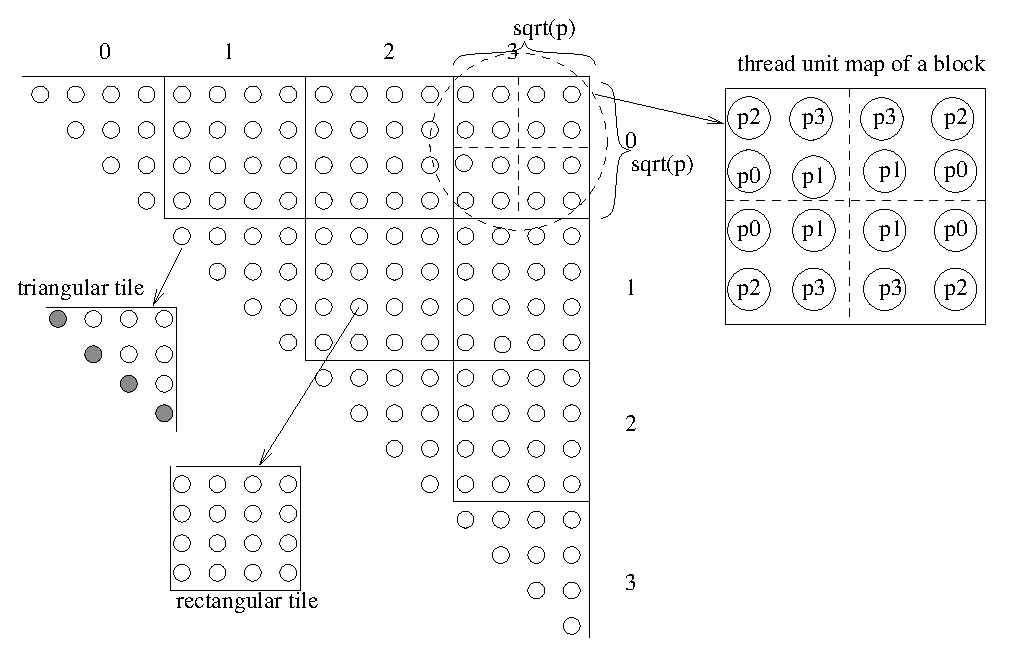
\includegraphics[width=5in,height=2.5in]{Img/Chap_Algorithm/blocked_pdp}
		\caption{细粒度并行算法的数据分块}
		\label{fig:blocked_pdp}
	\end{center}
\end{figure}

图\ref{fig:blocked_pdp}给出了分块的示例,每个块的大小是$4p$,没一条带的第一块是三角形,其他都是矩形。每个块又被划分成大小为$p=\sqrt{p}\times\sqrt{p}$的子块,子块中的元素映射到线程组成的二维网格。更进一步的优化是对矩阵分片,即每个子块的元素都是$x\times y$的片。以计算$A(0,3)$为例,第一部分的计算是$(A(0,1)\otimes A(1,3))\oplus(A(0,2)\otimes A(2,3))$,第二部分的计算是$(A(0,0)\otimes A(0,3))\oplus(A(0,3)\otimes A(3,3))$。第一部分计算表现除了两级并行性:一是$O(j-i-1)$ 个$\oplus$ 操作,二是其中的$\otimes$操作。而第二部分的计算由于两个连续块之间数据依赖关系的限制,并行度相对较底。本节提出的并行算法能够通过调控减少这部分计算。事实上,在计算第二部分的过程中,两个操作$A(i,i)\otimes A(i,j)$, $A(i,j)\otimes A(j,j)$ 都依赖于本身$A(i,j)$,这样把$A(i, i), A(j, j), A(i, j)$合成一个大的三角形矩阵,从而可以沿对角线方向上并行计算。
\begin{figure}[htbp]
	\begin{center}
		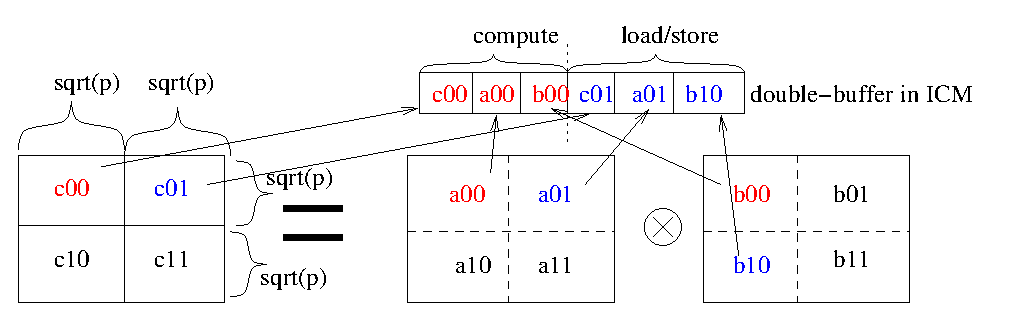
\includegraphics[width=4.5in,height=1.2in]{Img/Chap_Algorithm/sub_block}
		\caption{子块的计算}
		\label{fig:sub_block}
	\end{center}
\end{figure}

第二部分 $\oplus_{k=i+1}^{j-1}(A(i,k)\otimes A(k,j))$的计算中,每个$\otimes$操作能够并行执行。然而,问题是尽管对所有线程单元而言存储访问是一致的,但对不同存储层次的访问是不一致的,因此需要一种策略优化存储访问的开销,以利用片上大规模的线程单元获得高的扩展性。
由于每块大小是$2\sqrt{p}$,把每块又进一步划分成4个大小为$p=\sqrt{p}\times\sqrt{p}$的子块,子块中的每个元素映射到一个线程单元。当执行$\otimes$操作时,所有操作之间没有数据依赖关系,从而可以并行执行。对任何$i+1 \le k \le j-1$,需要计算$A(i,k)\otimes A(k,j)$。为了描述简便,用$C$、$A$和$B$ 分别表示$A(i, j)$、$A(i, k)$和$A(k, j)$。数据依赖关系要求$C$的一个子块的计算需要同一行、列上相应$A$和$B$的子块,这和矩阵乘的计算一样。一个子块的计算需要$(2\sqrt{p})^{3}\times(3+1)=32p\sqrt{p}$ (3 loads and 1 store)存储操作,而且存在数据重用。并行算法把所有线程单元划分成{\em computation}和{\em helper}线程。{\em helper}线程主要用于执行片内和片外存储之间数据移动存取操作,能够和{\em computation}执行计算操作同时进行。为了减少从片外存储读取操作的次数,算法采用double-buffering策略。在片内存储中分配三个double buffer,每个buffer存储其中某个子块的一半。这样,double buffer中,一半存储空间用于计算,一半用于缓存两个存储层次之间的数据交换。计算如图\ref{fig:sub_block}所示,该图演示了计算子块$C(0,0)$的存储映像。为了使{\em computation}和{\em helper}线程能够并行执行,需要满足当{\em computation}线程正在处理当前$C$的一个子块时,{\em helper}线程load/store用于计算$C$的下一个不同子块的数据。为了获得数据重用,$C$的四个子块的计算能够以流水的形式进行,流水过程包括8个并行操作。算法\ref{algo:psteps}描述了计算一个块的并行流水实现,每个操作步后需要一个同步操作以保证当前操作的load/store已经结束。

\begin{algorithm}\label{algo:psteps}
	{\bf ParllelSteps}\\
	startup: LOAD $C00$, $A00$, $B00$; \\
	step 1: COMPUTE $C00$; LOAD $A01$, $B10$;\\
	step 2: COMPUTE $C00$; LOAD $C01$, $B01$;\\
	step 3: COMPUTE $C01$; LOAD $B11$; STORE $C00$;\\
	step 4: COMPUTE $C01$; LOAD $C11$, $A10$;\\
	step 5: COMPUTE $C11$; LOAD $A11$; STORE $C01$;\\
	step 6: COMPUTE $C11$; LOAD $C10$, $B00$;\\
	step 7: COMPUTE $C10$; LOAD $B10$; STORE $C11$;\\
	step 8: COMPUTE $C10$; \\
	end: STORE $C10$;
\end{algorithm}

算法\ref{algo:psteps}需要4个对块$C$的load/stores操作,4个对$A$的load操作和6个对$B$的load操作,因此,计算块$C$需要$18p$个存储操作。尽管算法不能保证存储操作次数是最少的,但算法利用了计算和存储访问之间的并行,通过多线程隐藏了片外存储访问。而一个块$A(i,j)$的计算需要$O(j-i-1)$个$\otimes$操作,注意到算法中的{\em step 8},此时可以用一个{\em helper}
线程读入下一个$\otimes$操作需要的$C00$, $A00$, $B00$,这样,$O(j-i-1)$个$\otimes$操作也形成了流水形式。

如前所述,分片是提高局部性和控制通信粒度的有效策略,这里算法中的通信可以指访问片外存储操作。因此和优化Cache无关算法类似,动态规划矩阵分块对象是分片后的
矩阵。如图\ref{fig:blocked_pdp}所示,这里只考虑正方形片即片参数满足$x=y$。


\subsection{数据流体系结构中显式内存层次的优化}
渗透模型并行算法在IBM Cyclops64上实现并对最优分块因子进行了探索。IBM Cyclops64(C64)芯片是为IBM BlueGene/C千万亿次(PetaFlops)而设计的大规模多核结构,由于本研究的大量实验是在
该平台测试的,这里给出其体系结构的描述。如图\ref{fig:c64node}所示,一个C64芯片包含了80个处理器,每个处理器有两个线程单元(thread unit, TU),即一个芯片上集成了160个64位RISC处理核,5个处理器共享一个指令Cache,取代数据Cache的是分别配置成多个物理上局部的scratchpad
memory(SP)和所有处理单元共享的一致性存储访问的global
memory(GM)。一个芯片上还集成了4个DDR存储控制器以访问片外更多容量的DRAM。芯片内部所有处理单元之间通过crossbar网络互联,其每个端口的带宽达到384GB/s。

\begin{figure}[htbp]
	\centering
	% Requires \usepackage{graphicx}
	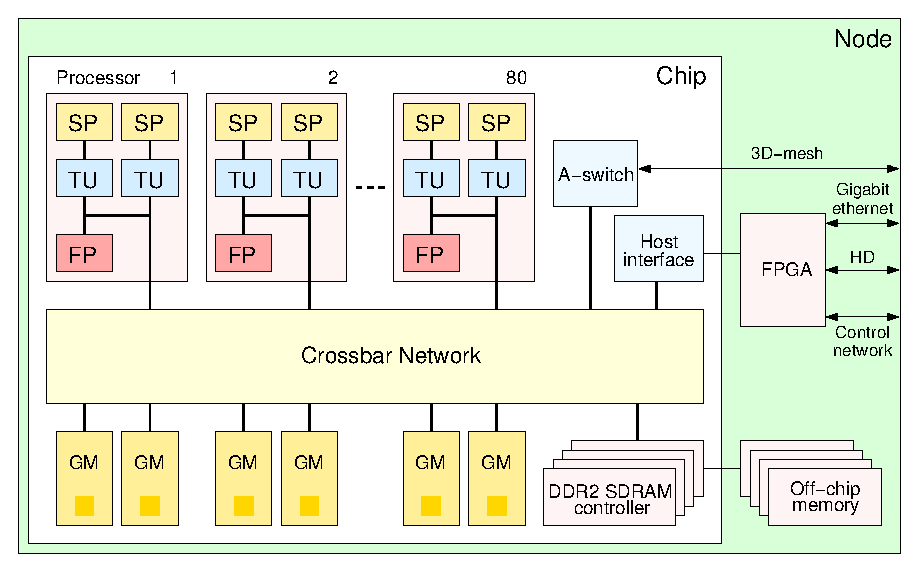
\includegraphics[width=5in,height=2.2in]{Img/Chap_Algorithm/c64node}\\
	\caption{IBM Cyclops64芯片结构}\label{fig:c64node}
\end{figure}
\begin{figure}[htbp]
	\centering
	% Requires \usepackage{graphicx}
	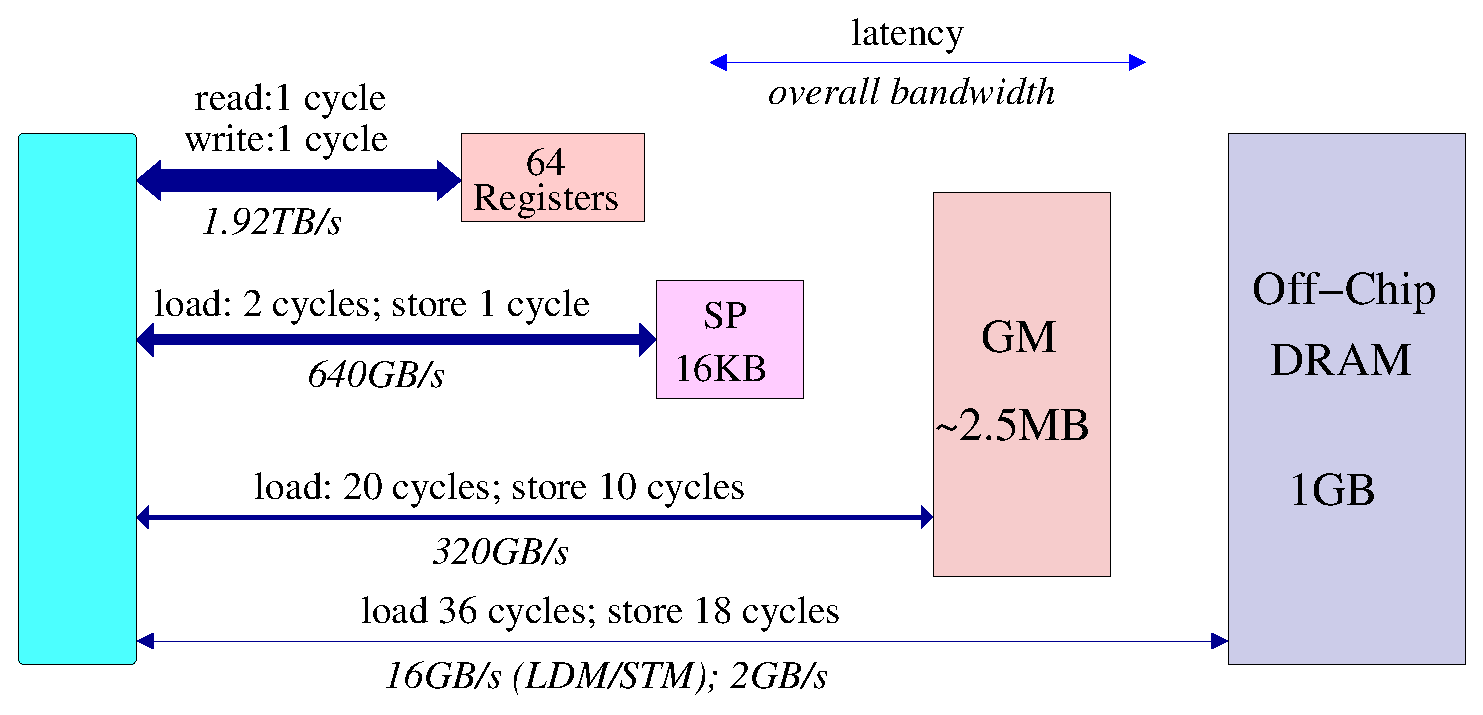
\includegraphics[width=5in,height=2in]{Img/Chap_Algorithm/c64-memory}\\
	\caption{IBM Cyclops64存储层次结构}\label{fig:c64-memory}
\end{figure}
总之,C64芯片体系结构有以下几个突出的特点:
\begin{itemize}
	\item 大规模处理单元、高速嵌入式存储和通信硬件集成到一个芯片上
	\item 支持大规模硬件多线程的有效执行
	\item 不支持虚拟存储管理,而是显式的三级存储层次:Scratchpad memory、on-chip SRAM和off-chip DRAM,
	所有的存储空间为所有的处理单元共享。片上SRAM的一部分配置成scratchpad
	memory,线程单元通过专用的数据通路快速访问自己局部的SP,访问其他线程单元局部的SP需要通过片上网络。其它on-chip
	memory即GM为所有线程单元
	共享并具有一致性存储访问性质,一个线程单元访问另外一个线程单元的SP和GM都需要通过片上crossbar网络。4个片内存储控制可以连接4个片外的大容量存储器,
	也配置成所有处理单元共享并具有一致性访问特点。当前的C64结构中片外DRAM是1GB。图\ref{fig:c64-memory}显示了该存储层次结构的延迟和带宽差异。
	\item 硬件支持barrier和细粒度同步操作
\end{itemize}

由于流水块操作$\otimes$是并行算法的主要计算部分,为了简化模型,
这里只考虑所有块操作$\otimes$的时间。基本的块操作$\otimes$由8个并行步骤组成。假设动态规划迭代空间大小为$n$,分片参数用$x$表示,线程个数用$p$表示。分片后
的迭代空间大小为$m=\frac{n}{x}$,然后对分片后的动态规划矩阵分块,每块大小为$4p=2\sqrt{p}\times
2\sqrt{p}$。这样,如果以块为单元,动态规划矩阵有$m'=\frac{m}{2\sqrt{p}}$行条带,一个行条带$i$有$m'-i$块。根据动态规划依赖关系,行条带$i$上的任何块
$A(i,j),(i\le
j<m'-i$的计算需要$j-i-1$个块操作$\otimes$。用符号$I_{\otimes}$表示整个计算过程所需要的块操作$\otimes$的个数:
\begin{displaymath}
I_{\otimes} = \sum_{i=1}^{m'-2}\sum_{j=i+1}^{m'-i-1}j %= \frac{m'(m'-1)(m'-2)}{3}
\end{displaymath}
因为$m=\frac{n}{x}$,代入上面的方程有:
\begin{equation}\label{eq:iters}
I_{\otimes} = \frac{1}{24}[\frac{n^{3}}{x^{3}p^{\frac{3}{2}}}-6\frac{n^{2}}{x^{2}p}+8\frac{n}{x\sqrt{p}}]
\end{equation}


\subsubsection{存储访问复杂性}
该并行算法的设计基于渗透模型,该模型和out-of-core模型类似,注意到out-of-core模型中用I/O复杂性衡量算法。在本研究中的大规模多核平台具有显式存储层次结构,
如图\ref{fig:c64-memory}所示,把最靠近硬件线程单元的SPM作为一级存储,片内SRAM作为二级存储,片外DRAM作为三级存储。由于SPM主要用于存放线程的状态和
栈等私有数据,一般不用于应用程序数据交换。这样,按照延迟容忍模型的规范,片内SRAM用于ICLM,片外DRAM用于OCM。这里的存储访问复杂性(memory-traffic
complexity)定义为远小于问题规模的片内SRAM和大于问题规模的片外DRAM之间存储访问的次数。从而,有如下引理:
\begin{lemma}\label{lemma:memory_complexity}
	采用分片后的并行流水算法\ref{algo:psteps},分片参数是$x$。其存储访问复杂性(memory-traffic complexity)减少了$x$倍,其中
	$x=O(\sqrt{C})$,$C$是片内SRAM大小。
\end{lemma}

\begin{proof}
	没有采用分片的并行算法,非流水和流水两种形式的存储访问复杂性分别为:
	\begin{displaymath}
	M_{non-pipeline} = I_{\otimes}\times 32p\sqrt{p} = O(n^{3})
	\end{displaymath}
	\begin{displaymath}
	M_{pipeline} = I_{\otimes}\times 18p = O(\frac{n^{3}}{\sqrt{p}})
	\end{displaymath}
	当对矩阵分片后,每个$\otimes$操作的元素是以大小为$x\times
	x$的片为单位。每个$\otimes$操作产生$x^{2}$次存储访问,因此一个块$\otimes$操作的存储访问次数是$18px^{2}$。考虑整个算法的块操作次数$I_{\otimes}$,得到分片后
	并行流水算法的存储访问复杂性为:
	\begin{displaymath}
	\begin{array}{ll}
	M_{tile} = I_{\otimes}\times 18p \\
	\hspace*{3pc}= \frac{1}{24}[\frac{n^{3}}{x^{3}p^{\frac{3}{2}}}-6\frac{n^{2}}{x^{2}p}+8\frac{n}{x\sqrt{p}}]\times 18p=O(\frac{n^{3}}{x\sqrt{p}})
	\end{array}
	\end{displaymath}
	证毕。
\end{proof}
引理\label{lemma:memory_complexity}给出了算法存储访问复杂性的上界,由于算法的基本操作$\otimes$和矩阵乘的计算行为一样,而且以前的研究证明了其存储访问
复杂性的下界为$\Omega(\frac{n^{3}}{x\sqrt{p}})$\cite{layout-tpds03},从而有下面关于在多核结构上的并行流水动态规划算法的存储访问复杂性定理:
\begin{theorem}
	分片的并行流水算法的存储访问复杂性是近似最优的。
\end{theorem}
存储访问复杂性的概念衡量了一个算法在通用体系结构上类似的存储访问次数。然而,注意到大规模多核结构中,“分离”出的{\em
	helper}线程专门用于存储访问以实现计算和片外存储访问的重叠,而且在有限的带宽内,{\em
	helper}的片外存储访问也可以并行。因此算法的设计要权衡需要多少个“分离”的{\em
	helper}线程。这里提出另外一个概念--存储访问效率(memory-traffic efficiency),定义为存储访问减少量和{\em
	helper}线程个数的比值。本节提出的并行流水算法使用了两个{\em
	helper}线程,其中一个用于load操作,另一个用于store操作,则4个store操作能够完全被重叠,导致时间的减少量为$4/18$,因此存储访问效率是11\%。但注意到
算法\ref{algo:psteps}中每个并行步最多只需要两个片外存储访问,如果不静态限定{\em helper}线程的操作,而是在某个{\em
	helper}线程空闲时去执行store操作,则4个load和4个store操作能够被隐藏,从而时间减少量为$8/18$,存储访问效率为22\%。如果使用3个{\em
	helper}线程,所有的片外存储访问操作能够并行执行,时间减少量为$10/18$,但存储访问效率是19\%。可以看出,存储访问效率取决于存储访问中的并行性,而且在实际
的平台上其并行性受带宽的限制,所以,使用更多的{\em helper}线程并不意味着高的性能。
\subsubsection{运行时间}
通过分片的并行流水算法分析,并行算法的运行时间受分片参数$x$的影响,本节构建关于最小化运行时间的性能分析模型以确定得到最少运行时间的分片参数$x$。假设
一个标准三重循环实现的动态规划的运行时间为$\alpha$,一次片外存储访问延迟为$\beta$。算法\ref{algo:psteps}的每一个步骤中,一个线程需要执行$\sqrt{p}$个
$\otimes$操作,这样,一个并行步的计算时间为:
\begin{displaymath}
T_{comp} = \alpha\sqrt{p}x^{3}
\end{displaymath}
如前面的分析,两个存储访问能够并行执行,片外存储访问的延迟为:
\begin{displaymath}
T_{tran} = \beta px^{2}
\end{displaymath}
由于{\em computation}线程和{\em
	helper}线程能够并行进行,相应地,片外和片内存储之间的数据传输和计算时间被重叠起来,因此,一个分片的基本操作$\otimes$的运行时间为:
\begin{equation}\label{eq:block_time}
T_{\otimes}=max\{T_{comp}, T_{tran}\}=max\{\alpha\sqrt{p}x^{3},\beta px^{2}\}
\end{equation}
合并方程\ref{eq:iters}和\ref{eq:block_time},得到并行流水算法的运行时间:
\begin{equation}\label{eq:execution}
\begin{array}{ll}
T_{0}(x) = \frac{n}{2x\sqrt{p}}\times2\beta px^{2}+I_{\otimes}\times 8\times T_{\otimes}\\
=n\beta\sqrt{p}x+8\times I_{\otimes}\times max\{\alpha\sqrt{p}x^{3},\beta px^{2}\}\\
=\left\{ \begin{array}{ll} T_{1}(x)=n\beta\sqrt{p}x+8I_{\otimes}\times\beta px^{2} &
\textrm{$x<\frac{\beta\sqrt{p}}{\alpha}$}\\
T_{2}(x)=n\beta\sqrt{p}x+8I_{\otimes}\times\alpha\sqrt{p}x^{3} & \textrm{$x\ge\frac{\beta\sqrt{p}}{\alpha}$}
\end{array} \right.
\end{array}
\end{equation}
对角线上的三角形块是自我闭包的,其运行时间为:
\begin{equation}\label{eq:tri}
T_{3}(x)=(\sum_{i=1}^{m'}i\times\sum_{j=1}^{4\sqrt{p}}+m'\sum_{j=1}^{2\sqrt{p}})x^{3}\alpha =n\alpha
px^{2}+\frac{n^{2}\alpha(4\sqrt{p}+1)}{4}x
\end{equation}
因此,选择最优的分片参数即为解下面的优化问题:
\begin{equation}\label{eq:all}
\begin{array}{ll}
\mathcal{P}:Minimize\hspace*{1pc}T(x)=T_{0}(x)+T_{3}(x) \\
\hspace*{4pc} s.t. \hspace*{1pc}\frac{\beta\sqrt{p}}{\alpha}\le x<min\{\sqrt{\frac{C}{48p}},\frac{n}{4\sqrt{p}}\}
\end{array}
\end{equation}
该优化问题的目标是求解最优的分片参数$x$以最小化函数$T(x)$。为了解该非线性优化问题,需要先给出并证明两个推论。注意到目标函数满足下列属性:
\begin{displaymath}
\begin{array}{ll}
T_{1}(x) \ge T_{2}(x) & \textrm{$x\le\frac{\beta\sqrt{p}}{\alpha}$}
\end{array}
\end{displaymath}
\begin{displaymath}
\begin{array}{ll}
T_{1}(x) = T_{2}(x) & \textrm{$x=\frac{\beta\sqrt{p}}{\alpha}$}
\end{array}
\end{displaymath}
\begin{displaymath}
\begin{array}{ll}
T_{1}(x) \le T_{2}(x) & \textrm{$x\ge\frac{\beta\sqrt{p}}{\alpha}$}
\end{array}
\end{displaymath}
这样,优化问题转化为:
\begin{equation}\label{eq:opt}
\begin{array}{ll}
\mathcal{P_{0}}:\hspace*{1pc}Minimize\hspace*{1pc}T_{0}(x) = 8\times min\{max\{T_{1}(x), T_{2}(x)\}\} \\
\hspace*{3pc}s.t.\hspace*{1pc}\textrm{$x=O(\sqrt{C})$}
\end{array}
\end{equation}
在并行流水算法中,片内SRAM至少有6个大小为$p$个片的存储块用于数据交换实现double-buffering,其元素数据类型是{\em double},从而得到下面的限制条件:
\begin{equation}\label{eq:c1}
x < \sqrt{\frac{C}{48p}}
\vspace{-0.225cm}
\end{equation}
另外,由于$I_{\otimes}>0$,推导出第二个限制条件:
\begin{equation}\label{eq:c2}
x < \frac{n}{4\sqrt{p}}
\end{equation}
综上,结合方程\ref{eq:iters}、\ref{eq:opt}、 \ref{eq:c1}和 \ref{eq:c2},非线性优化问题表示如下:
\begin{equation}\label{eq:opt_inst}
\begin{array}{ll}
\mathcal{P'}:\hspace*{1pc}Minimize\hspace*{1pc}T_{0}(x) \\
=\frac{1}{24}\left\{ \begin{array}{ll} T_{1}(x)= \frac{n^{3}\beta}{\sqrt{p}x}+9n\beta\sqrt{p}x-6n^{2}\beta &
\textrm{$x\le\frac{\beta\sqrt{p}}{\alpha}$}\\
T_{2}(x)= 8n\alpha x^{2}+(n\beta\sqrt{p}-\frac{6n^{2}\alpha}{\sqrt{p}})x+\frac{n^{3}\alpha}{p} &
\textrm{$x\ge\frac{\beta\sqrt{p}}{\alpha}$}
\end{array} \right. \\
\hspace*{3pc}s.t.\hspace*{1pc}\textrm{$x<\sqrt{\frac{C}{48p}}$} \\
\hspace*{4pc}\hspace*{1pc}\textrm{$x<\frac{n}{4\sqrt{p}}$}
\end{array}
\end{equation}
最优问题的解用$x^{*}$表示,现在证明推论\ref{cor:solution1}。
\begin{corollary}\label{cor:solution1}
	给定问题规模$n$和片内SRAM大小$C$,优化问题$\mathcal{P"}$的最优解$x^{*}$为:
	\begin{displaymath}
	x^{*}=\left\{\begin{array}{ll} \lfloor\frac{n}{4\sqrt{p}}\rfloor-const & \textrm{$n\le\sqrt{\frac{C}{3}}$} \\
	\lfloor\sqrt{\frac{C}{48p}}\rfloor-const & \textrm{$n\ge\sqrt{\frac{C}{3}}$}
	\end{array}\right.
	\end{displaymath}
	其中$const$是一个使$x^{*}>0$的常数。
\end{corollary}
\begin{proof}:
	$T_{1}(x)$和$T_{2}(x)$的解分别用$x_{1}^{*}$和 $x_{2}^{*}$表示,它们满足如下关系:
	\begin{displaymath}
	x_{1}^{*}=\frac{n}{3\sqrt{p}} \hspace*{2pc}x_{2}^{*}=\frac{6n\alpha-p\beta}{16\alpha\sqrt{p}}
	\end{displaymath}
	设$x_{mid}^{*}=\frac{\beta\sqrt{p}}{\alpha}$把优化问题的解空间划分成两部分:$(0,
	x_{mid}^{*}]$和$[x_{mid}^{*}, min\{\sqrt{\frac{C}{48p}},\frac{n}{4\sqrt{p}}\})$。显然,
	$x_{1}^{*}>\frac{n}{4\sqrt{p}}$和$x_{2}^{*}>\frac{n}{4\sqrt{p}}$表明$x_{1}^{*}$和$x_{2}^{*}$ 已经超出了解空间,在解空间中,位于$x_{1}^{*}$和$x_{2}^{*}$左边时,$T_{1}(x)$和$T_{2}(x)$ 是递减的且在$min\{\sqrt{\frac{C}{48p}},\frac{n}{4\sqrt{p}}\}-const$时达到最小值。
\end{proof}
\begin{corollary}\label{cor:solution2}
	给定问题规模$n$而且$2<p<\frac{\alpha}{\beta}min\{\sqrt{\frac{C}{48}},\frac{n}{4}\}$,优化问题$\mathcal{P}$的解为
	$x^{*}=\frac{\beta\sqrt{p}}{\alpha}$ 
\end{corollary}
\begin{proof}
	设$a=(8n\alpha+n\alpha p)$,$b=(n\beta\sqrt{p}-\frac{6n^{2}\alpha}{\sqrt{p}}+\frac{n^{2}\alpha(4\sqrt{p}+1)}
	{4})$,当$x^{*}=\frac{-b}{2a}$,$T(x)$取得全局最小值。然而,解空间的区间为[$\frac{\beta\sqrt{p}}{\alpha}$, $min\{\sqrt{\frac{C}{48p}},\frac{n}{4\sqrt{p}}$\})。假设$x^{*}>
	\frac{\beta\sqrt{p}}{\alpha}$,有:
	\begin{equation}\label{eq:theorem2}
	n<\frac{4\beta p(2p+17)}{24\alpha-\alpha\sqrt{p}(4\sqrt{p}+1)}
	\end{equation}
	根据方程\ref{eq:theorem2},$n>0$ 当且仅当 $p\le 2$。也就使说,$p>2$而且$x^{*}<\frac{\beta\sqrt{p}}
	{\alpha}$。一元二次方程的属性表明当 $x>x^{*}$时,$T(x)$递增。优化问题$\mathcal{P}$的解为$\frac{\beta\sqrt{p}}{\alpha}$
\end{proof}
根据推论\ref{cor:solution1}和\ref{cor:solution2},得到下面求解最优分片问题中分片参数的定理:
\begin{theorem}\label{thm:solution}
	分片并行流水动态规划算法的最优分片参数由如下规则确定:
	如果$2<p<\frac{\alpha}{\beta}min\{\sqrt{\frac{C}{48}},\frac{n}{4}\}$,
	$x^{*}=\frac{\beta\sqrt{p}}{\alpha}$;
	否则,
	\begin{displaymath}
	x^{*}=\left\{\begin{array}{ll} \lfloor\frac{n}{4\sqrt{p}}\rfloor-const & \textrm{$n\le\sqrt{\frac{C}{3}}$} \\
	\lfloor\sqrt{\frac{C}{48p}}\rfloor-const & \textrm{$n\ge\sqrt{\frac{C}{3}}$}
	\end{array}\right.
	\end{displaymath}
\end{theorem}
\begin{figure}[!htbp]
	\begin{center}
		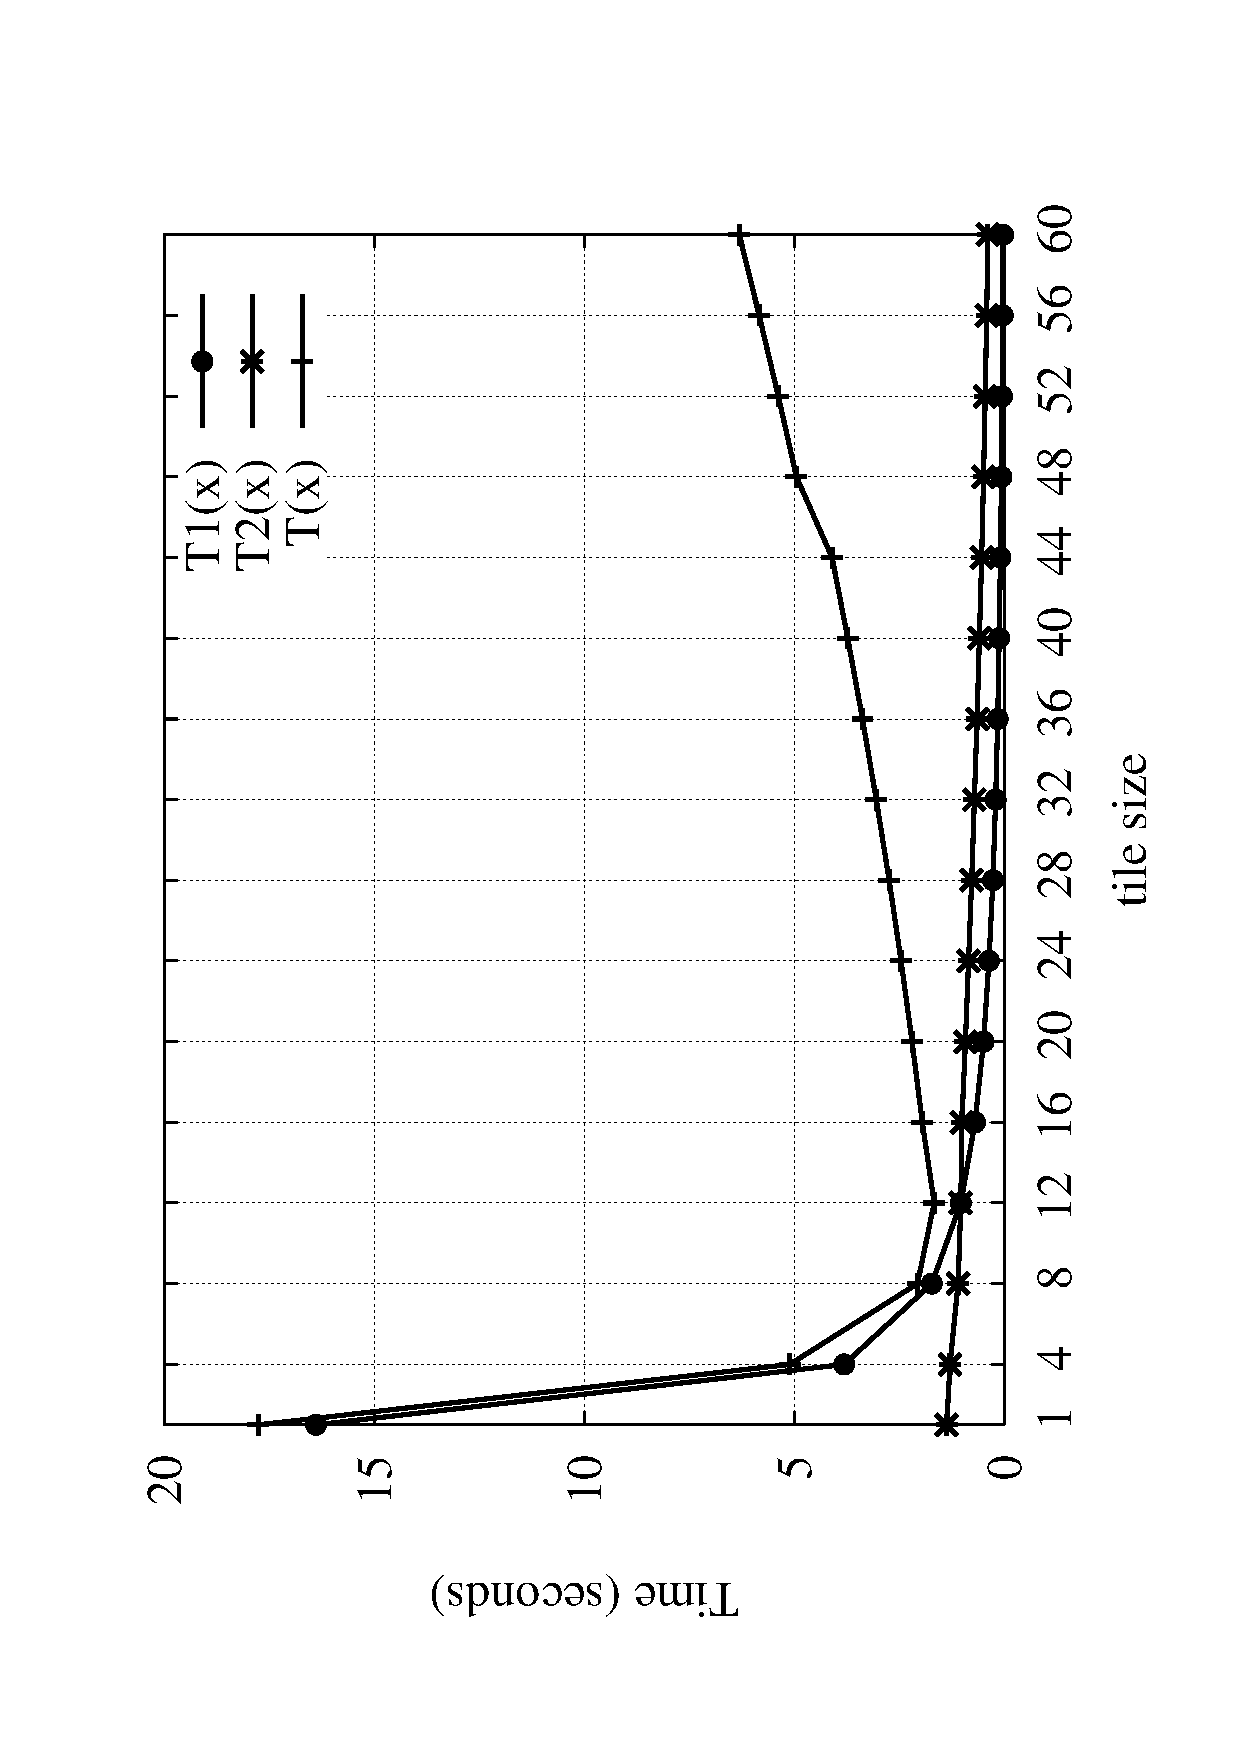
\includegraphics[scale=0.6]{Img/Chap_Algorithm/model}
		\caption{最优分片的理论分析}
		\label{fig:model}
	\end{center}
\end{figure}

图\ref{fig:model}给出了问题规模是$n=1024$在$p=16$时的最优解,根据定理\ref{thm:solution}在$p=16$,$n=1024$的最优解。其中  $x_{mid}^{*}=12$
$min\{\sqrt{\frac{C}{48p}},\frac{n}{4\sqrt{p}}\}=64$, $x^{*}=12$。
$T_{0}(x)$的解说明$x$越大越好,然而增加$x$的值导致计算并行度底的三角形部分的计算增加。事实上,前述优化问题解能够解释并行算法的扩展性。$x_{mid}^{*}$把解空间划分成两部分。当最优解落入左边区间时,即$\frac{n}{p}<\frac{\beta}{\alpha}$,说明当线程数量超过一定值时,程序的执行时间由存储数据传输决定。推论\ref{cor:solution1}证明了最优解位于$x_{mid}^{*}$的右边,这说明并行算法的扩展性主要取决与计算操作数量,而不是存储访问延迟。因此,本研究提出的并行流水算法在具有显式存储的大规模多核体系结构上有较好的扩展性。

\begin{table}
	\begin{center}
		\caption{不同问题规模下的运行时间(效率)。单位: 秒(seconds)} \label{tab:exe_time}
		\begin{tabular}{|l|l|l|l|l|l|}
			\hline
			\#threads & 256 & 512 & 1024 & 2048 & 4096 \\\hline
			serial & 1.40 & 11.28 & 90.43 & 226.54 & 1738.88\\\hline
			4 & 0.36 & 2.46 & 17.94 & 42.72 & 275.82\\\hline
			16 & 0.16 & 1.01 & 6.99 & 15.75 & 106.28\\\hline
			64 & 0.12 & 0.62 & 4.57 & 7.57 & 44.06\\\hline
		\end{tabular}
	\end{center}
\end{table}
表\ref{tab:exe_time}总结了串行程序和并行程序的运行时间,数据显示并行算法获得了近似线性的加速比。算法\ref{algo:psteps}的并行流水计算策略提高数据重用,减少了片外存储的访问次数,从而大大降低了存储访问的开销。通过以前的算法理论分析,片外存储访问数量能够被减少近似3倍,但注意到算法采用了分片技术进一步提高程序运行时的局部性,所以性能提高要略大于3倍。该并行流水算法通过增加数据重用而优化了访问片外存储的带宽。同时,IBM Cyclops64也支持同时多个存储load/store操作的指令,如LDM/STM指令由4个LDD/STD(load/store double word)实现,因此,如果程序能够使用这些指令,则理想情况下带宽利用可以增加将近4倍。




\section{大数据分析-高性能图遍历算法}\label{sec:PM_graph}

本节介绍对大数据分析应用中的图计算问题的基于渗透模型的并行算法设计和优化。首先给出大规模网络分析算法介度中心(betweenness centrality)的图计算算法。然后,基于渗透模型的流水线算法实现框架,描述并行介度中心图遍历算法。进一步,利用数据流体系结构中硬件同步机制的支持优化图计算问题。

\subsection{图遍历算法介绍}
大规模网络分析方法应用于许多重要的应用中如社会网络分析(亲朋关系、组织结构和反恐)、WWW因特网(网络拓扑)、交通运输网络、家谱关系和生物信息学
(蛋白质相互作用网络、性/AIDS网络和食物网络)\citep{network-app-social-Freeman,network-app-social-url,network-cs-acm,network-cs-connections,network-app-web,network-app-internet,network-app-bioinformatics,network-app-nature,network-app-recomb,network-app-aids}。在大多数应用中,图的抽象和算法经常用于描述和解释问题的本质\cite{network-app,network-app-sci}。基于图论的网络分析能够从
真实数据构建的大规模图来抽取有意义的信息,如识别反恐网络中关键人物、蛋白质网络中起主要调控作用的蛋白等。

构建合适的模型模拟复杂的真实世界网络本身就是一个
相当重要而活跃的研究课题\citep{network-model-nas, network-model-globcomm,network-model-rmat}。在过去的几十年中,随机网络(random
networks)\citep{network-model-nas}模型一直是大规模网络分析的主要研究工具。构建一个图时,每个顶点的度$k$服从某个概率分布$P(k)$。在随机图中,由于每个顶点的边数随机选择,
大多数顶点的度几乎一样。然而,最近的大量研究表明许多复杂的网络系统显示出有组织的结构。人们又提出了Scale-Free(SF)网络模型\citep{network-sf-math,network-sf-phy}。SF网络中的顶点的度服从幂律(power-law)分布\citep{network-power-law},即:
\begin{equation}\label{eq:power_law}
P(k)\sim k^{-\gamma}
\end{equation}
和SF网络模型匹配的网络分析应用有WWW因特网、蛋白质相互作用网络和性/AIDS网络等。与随机网络中度的均匀分布不同,SF网络中绝大多数顶点只有很少的连接,只有
少数几个顶点有许多的连接。

分析大规模网络的一个最重要的工具是图的向心性指标(centrality
index)\citep{network-centrality}。社会网络分析中,顶点的向心性用来给所有的参与者分级和区别最主要的参与者;在蛋白质网络中,蛋白质的向心性识别具有高度互联的一组蛋白质,这些蛋白质
在调控相互作用中扮演主要角色。到目前为止,已经有多个向心性指标用于分析网络特征,其中最重要的一个就是
介度中心(betweenness centrality)\citep{network-bc}。

用图$G=(V,E)$表示一个网络结构,其中$V$是顶点集合,$E$是边集合。顶点和边的数量
分别用$n$和$m$表示,图可以是有向或者无向的。每一条边赋予一个权值$w(e)$(无权图中$w(e)=1$)。从顶点$s$到$t$的路径用多个有序的二元组
$<u_{i},u_{i+1}>$表示,其中$0\le i\le l, u_{0}=s, u_{t} =
t$,路径的长度$d(s,t)$是该路径上所有边的权值的和。用$\sigma_{st}$表示顶点$s$和$t$之间最小路径的条数,而其中经过另外一个顶点$v$的最小路径条数用
$\sigma_{st}(v)$表示。1977年,Freeman\cite{network-bc}首次提出了介度中心概念。用$\delta_{st}(v)$表示任意顶点的两两依赖性(pairwise
dependency),即顶点$s$到$t$之间的最小路径中经过顶点$v$的条数与总数的比值:
\begin{equation}\label{eq:pairwise_dep}
\delta_{st}(v)=\frac{\sigma_{st}(v)}{\sigma{st}}
\end{equation}
任意一个顶点$v$的介度中心(betweenness centrality)定义如下:
\begin{equation}\label{eq:bet_cent}
BC(v)=\sum_{s\ne v\ne t\in V}\delta_{st}(v)
\end{equation}
介度中心的值度量一个顶点在网络中交互的控制地位,辨别出其中关键的部分。高的介度中心值表明该顶点通过相对较短的最小路径达到其他顶点,即该顶点在连接其他
顶点的路径中是更关键的部分。直接计算所有顶点的介度中心值的算法如下:
\begin{enumerate}
	\item 计算任意顶点对$(s,t)$之间的最小路径长度和数量;
	\item 对每一个顶点$v$,计算所有可能的两两依赖性$\delta_{st}(v)$,然后求和。
\end{enumerate}
通过Floyd-Warshall算法计算所有顶点对之间最小路径算法,该直接计算的时间复杂度是$O(n^{3})$。基于Dijkstra单源最小路径算法和宽度优先搜索(breadth
first search)算法,通过消除计算过程中的冗余计算,Brandes\citep{brandes-bc}提出了一种时间复杂度为$O(mn+n^{2}logn)$的快速算法。

定义从$s$出发的最短路径上一个顶点$v$的前驱集合:
\begin{equation}
P_{s}(v)=\{u\in V: \{u,v\}\in E, d(s,v)=d(s,u)+d(u,v)\}
\end{equation}
为了消除计算所有两两依赖性的冗余部分,增加一个中间变量$\delta_{s}(v)$表示源顶点$s\in V$对其最短路径上某个顶点$v\in
V$的依赖性:
\begin{equation}
\delta_{s}(v)=\sum_{t\in V}\delta_{st}(v)
\end{equation}
Brandes算法较少计算量的最重要观察是$\delta_{s}(v)$满足如下的递归关系:
\begin{equation}\label{eq:delta}
\delta_{s}(v)=\sum_{w:v\in P_{s}(w)}\frac{\sigma_{sv}}{\sigma_{sw}}(1+\delta_{s}(w))
\end{equation}
$\delta_{s}(v)$事实上是$BC(v)$的部分中间结果值,最后,$BC(v)$的计算表示如下:
\begin{equation}\label{eq:BC}
BC(v)=\sum_{s\neq v\in V}\delta_{s}(v)
\end{equation}
和动态规划求解问题类似,计算介度中心算法也明显分为两个连续阶段:向前BFS得到最小路径(后面简称BFS)和向后累加依赖性值(简称回溯)。
\begin{enumerate}
	\item {\bf BFS:}在BFS阶段, 对每一个顶点$s\in
	V$遍历图搜索最小路径,同时保留所有最小路径上的顶点的前驱集合$P_{s}(v)$和经过中间顶点$w$的最小路径的条数$\sigma(w)$。
	\item {\bf 回溯:}对每一个源顶点$s$,使用其最小路径树的信息如经过中间顶点$w$的最短路径条数$\sigma(w)$和前驱集合,根据递归
	式\ref{eq:delta}计算$\delta_{s}(v)$。最后累加所有部分值得到顶点$v$的介度中心值。
\end{enumerate}

尽管图分析算法广泛应用于大量重要的实际问题中,然而由于其相当不规则的计算特征,导致大多数的图算法不同于传统的科学计算,不能够采用常规的优化策略提高
程序运行性能。图算法区别与多数传统科学计算的非规则特点如下:
\begin{itemize}
	\item {\bf
		很少的局部性和数据重用:}真实世界的网络规模巨大,通常有上百万甚至上亿顶点和边。如何设计空间有效的数据结构存储大规模数据表示就是一个极具挑战性的问题,
	并行外部算法设计(out-of-core
	algorithms)已经证明了在一定情况下是一种可行的策略。然而,这种策略要求数据结构是可以划分的,这对大多数规则的科学计算问题相当适合;但模拟真实世界
	网络的图结构由于其高度非结构性而通常不可简单划分。图中每个顶点的度也是分布不均,如本研究中SF图模型。这种非结构性的度分布也导致了程序在存储访问时
	可变的步长和随机性,从而很难在基于Cache存储结构上获得局部性。通常,在一次图遍历的过程中,一个顶点只需要访问一次,这样几乎不存在数据重用。
	\item {\bf
		动态非连续存储访问:}事实上,大多数的图算法中计算操作相对存储访问的比例很低,而且存储访问模式不能够静态地确定。例如,图遍历算法按级访问所有顶点,
	下一级需要访问的顶点是在当前一级遍历时动态确定的。也就是说,存储访问模式是动态数据相关的,这样,常规的体系结构上的预取机制不能有所帮助。而且由于
	两个顶点的邻接关系也是动态随机生成的,导致大量的非连续的存储访问。
	\item {\bf
		细粒度并行性:}遍历图通常按级进行,但级之间存储数据依赖关系,所以不能在级之间实现粗粒度并行。遍历一个顶点的所有邻接点时,可能存在并行访问的
	情况。但相对于大规模并行计算机,这种并行性是细粒度的,特别是对稀疏图如SF图模型。在同一级,如果有多个顶点,遍历这些顶点的邻接点可能可以并行进行,
	但如果两个顶点共享一个邻接点时,需要同步机制保证冲突访问。
\end{itemize}

大多数常规的基于Cache并行计算机体系结构的设计出自程序中具有高度局部性、规则存储访问模式和强调计算操作的粗粒度并行,显然,图算法这些源于非规则的计算行为的特征限制了在目前常规并行体系结构上获得高的加速比和好的可扩展性。


\subsection{渗透模型的流水算法设计}
把BFS阶段访问一个顶点的邻接点的操作称为扩展,当前需要扩展的顶点保存在一个队列中。

\begin{figure}[htbp]
	\begin{center}
		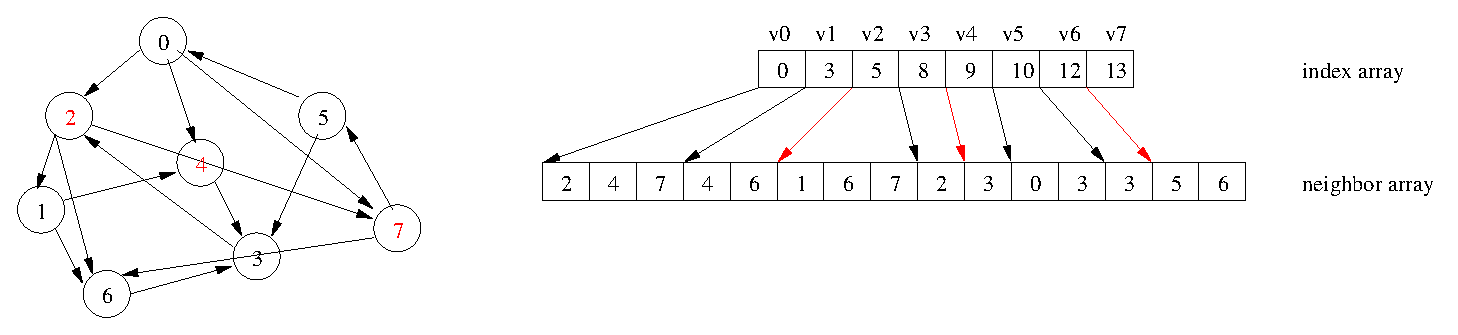
\includegraphics[width=6in,height=1.5in]{Img/Chap_Algorithm/adjacent}
		\caption{邻接数组数据结构}
		\label{fig:adjacent}
	\end{center}
\end{figure}

由于需要分析的图是稀疏图,算法采用存储空间有效的数据结构-邻接数组(adjacent array)来表示稀疏SF图,如图\ref{fig:adjacent}所示。邻接数组由两个数组组成:索引数组(index array)和邻接数组(neighbor array)。索引数组中的第$i$个元素表示顶点$i$的邻接点连续存储在邻接数组中偏移位置。当访问一个顶点的邻接点时,由于其邻接点是连续存储的,当顶点的度较高时,基于Cache体系结构上的预取或者分块技术可能可以优化性能,然而,稀疏SF图中绝大多数顶点的度都很低。两个不同顶点的邻接点的存储可能不是连续的,预取的邻接点可能不是即将要访问的顶点,这样不仅出现预取无效,而且导致大量Cache不命中,从而大大降低了程序的性能。介度中心算法还需要4个数据结构存储BFS树和每个顶点的介度中心值。存储前驱顶点的数据结构和邻接数组一样,表示$d, \sigma, \delta$分别是大小为$n$的线性数组。三个数组的访问模式取决于邻接点的访问,存储在邻接数组中的顶点序号可能不连续,事实上是一种随机分布状况(如图\ref{fig:adjacent}),因此,对三个数组的访问具有随机行为。显然,使用预取优化技术不能有任何帮助。
预取和猜测执行获得局部性依赖于存储访问的连续性或者规则的步长。scale-free稀疏图中顶点的度变化的。假设顶点$v_{2}, v_{4}, v_{7}$保存在队列中,在邻接数组中,$v_{2}, v_{4}, v_{7}$的邻接点存放在不连续的区域,而且对$d,\sigma,\delta, BC$数据结构的访问几乎是随机的,例如当扩展$v_{2}, v_{4}, v_{7}$时,访问序列是$d[1],d[6],d[7],d[3],d[5],d[6]$($\sigma$也是一样)。对$d,\sigma,\delta, BC$访问依赖于邻接数组,而且这种依赖关系是随着运行时变化的,这样的动态非连续存储访问模式不能从预取或者预测技术中获得性能提高。

为了利用动态的局部性,需要对非规则计算的局部性行为新的分析。注意到介度中心计算程序中存在非连续局部性,但是这些局部性离散地出现程序的执行中。然而大多数体系结构(包括众核)主要是利用连续局部性,因此在计算需要时及时把非连续局部性转换成连续局部性。例如,当$v_{2}, v_{4}, v_{7}$在当前队列中,顶点$v_{2}$的扩展操作需要把$v_{1}, v_{6}, v_{7}$读入到片内存储中。$v_{1}, v_{6}, v_{7}$连续存放中邻接数组中,然而$d[1],d[6],d[7]$是非连续的。基于渗透模型,在计算操作访问$d[1],d[6],d[7]$之前把这些离散的存储位置转换成连续的存储块,计算操作能够获得空间局部性,也就是说创建了即时局部性。

为了表述简单,这里只给出对邻接数组优化的算法描述。在算法\ref{algo:bc}中,BFS和回溯的主要存储操作是从队列/栈中读取顶点。
算法可能读取同一级上不同顶点的邻接点,因此存在不连续的存储访问。基于片内存储的低延迟和高带宽,算法优化可能从以下几个方面考虑:
\begin{itemize}
	\item 把对片外离散存储访问转换成对片内连续存储访问
	\item 分解并行任务以实现不同级存储访问之间的重叠
	\item 开发更多的片内计算和存储访问的并行
\end{itemize}
在多级并行算法,所有线程划分成若干组,线程组实现粗粒度并行,组内的线程实现中粒度和细粒度并行。粗粒度并行中,从一个源顶点开始的BFS为一个任务。线程组内的所有线程协作处理同一个任务。用$S_{i}$表示线程组$i$的源顶点。算法\ref{algo:bc}是多级并行算法的伪代码。

BFS按级遍历图,两个连续级之间存在数据依赖关系,即第$i+1$级的顶点是第$i$级顶点的第一次被访问的邻接点。和其它BFS并行算法一样,这里采用按级同步计算以保持数据依赖关系。然而,算法\ref{algo:bc}结合了中粒度和细粒度并行。当在选择第$i$级顶点的第一次访问的邻接点完成时,新形成的第$i+1$级的顶点继续在组内线程之间划分。第$i$级顶点用$V_{i} = \{v_{i1}, v_{i2}, ..., v_{in}\}$表示,每个顶点$V_{ij}$的邻接点为 $W_{j} = \{w_{j1}, w_{j2}, ..., w_{jm_{j}}\},1 \le j \le n$。算法把同一级的所有邻接点集合组合成一个更大的集合$NW_{i} = \bigcup_{1\le j\le n}W_{j}$,然后在同一个线程组内分配$NW_{i}$。由于可能存在平行边和两个不同的顶点对应同一个邻接点,即可能存在两个线程同时访问同一个邻接点。这样,需要同步机制如锁同步保护计算距离$d[w]$和记录路径信息$\sigma[w],P[w]$。

回溯过程和BFS类似,假设第$i$级有$n$个顶点$W_{i} = \{w_{i1}, w_{i2}, ..., w_{in}\}$ ,每个顶点的前驱为 $V_{j} = \{v_{j1}, v_{j2}, ..., v_{jm_{j}}\},1 \le j \le n$。同样,组合所有的前驱集合$PV_{i} = \bigcup_{1\le j\le n}P_{j}$并在一个组内线程之间划分。由于不同线程可能访问同一个前驱,同步机制需要保护对部分结果值$\delta(v)$的计算。最后,一个并行归约操作累加所有线程得到的部分结果值。
\begin{algorithm}\label{algo:bc}
	{\bf betweenness centrality}\\
	%{\bf Input:} G(V, E)\\
	%{\bf Output:} Array BC[1...n], where BC[v] gives the centrality metric for vertex v\\
	%1{\bf for } all $v\in V$ {\bf pardo}\\
	1\hspace*{1pc}$BC_{i=1...n}[v] = 0$ \\
	2{\bf for} all $s\in S_{i}$ {\bf do}\\
	3\hspace*{1pc}$P[w]\leftarrow$ empty list, $w\in V$\\
	4\hspace*{1pc}$\sigma[t]\leftarrow 0, t\in V;\sigma[s]\leftarrow 1;$\\
	5\hspace*{1pc}$d[t]\leftarrow -1,t\in V;d[s]\leftarrow 0$\\
	6\hspace*{1pc}Q$\leftarrow$empty queue\\
	7\hspace*{1pc}level = 0\\
	8\hspace*{1pc}enqueue $s\leftarrow Q_{level}$\\
	9\hspace*{1pc}{\bf while} $Q_{level}$ not empty {\bf do}\\
	10\hspace*{2pc}$NW_{level}$ $\leftarrow$ neighbors($\{v_{level,1},v_{level,2},...,v_{level,n}\}$, $Q_{level}$)\\
	11\hspace*{2pc}{\bf for} $w \in NW_{level}$ {\bf pardo}\\
	12\hspace*{3pc}{\it lock;}\\
	13\hspace*{3pc}{\bf if} $d[w]<0$ {\bf then}\\
	14\hspace*{4pc}enqueue $w\rightarrow Q_{level+1}$\\
	15\hspace*{4pc}$d[w]\leftarrow d[v]+1$\\
	16\hspace*{3pc}{\bf if} $d[w]=d[v]+1$ {\bf then}\\
	17\hspace*{4pc}$\sigma[w]\leftarrow \sigma[w]+\sigma[v]$\\
	18\hspace*{4pc}append $v\rightarrow P[w]$\\
	19\hspace*{3pc}{\it unlock;}\\
	20\hspace*{2pc}level = level+1;\\
	21\hspace*{2pc}{\bf sync};\\
	22\hspace*{1pc}$\delta[v]\leftarrow 0, v\in V$;\\
	23\hspace*{1pc}level = leve-1;\\
	24\hspace*{1pc}{\bf while} $level \ge 0$ {\bf do} \\
	25\hspace*{2pc}$PV_{level}\leftarrow predecessors(\{w_{level,1},w_{level,2},...,w_{level,n}\}, Q_{level})$\\
	26\hspace*{2pc}{\bf for} $v\in PV_{level}$ {\bf pardo}\\
	27\hspace*{3pc}{\it lock;}\\
	28\hspace*{3pc}$\delta[v]\leftarrow\delta[v]+\frac{\sigma[v]}{\sigma[w]}(1+\delta[w])$\\
	29\hspace*{3pc}{\it unlock;}\\
	30\hspace*{2pc}{\bf if} $w\neq s$ {\bf then}\\
	31\hspace*{3pc}{\it lock;}\\
	32\hspace*{3pc}$BC_{i}[w]\leftarrow BC_{i}[w]+\delta[w]$\\
	33\hspace*{3pc}{\it unlock;}\\
	34\hspace*{2pc}level = level - 1;\\
	35\hspace*{2pc}{\bf sync};\\
	36\hspace*{1pc}ParReduction(BC, $BC_{i}$)
\end{algorithm}

算法中的不同顶点的邻接点的组合提供了额外的并行。由于片内存储相对较小,当访问一个顶点的邻接点时,需要从片外存储中读入小部分顶点到片内存储中,这样,转换片外离散存储访问成片内连续存储访问的过程自然地被分成多个子任务。为了实现多个不同级存储访问之间的重叠,算法采用了double-buffering策略。线程分为{\em computation}线程和{\em helper}线程。{\em helper}线程用于在片外和片内存储中load/store数据,{\em computation}线程只有当数据在片内存储中时才开始执行,意味着{\em computation}线程主要访问片内存储。算法\ref{algo:db}给出了算法描述。为了处理当一个顶点的部分邻接点读入而buffer已经满的情况,算法需要记录访问邻接数组中的动态偏移。与基于DMA异步传输不同,这里的隐藏存储访问延迟的{\em helper}线程分为{\em load}线程和{\em store}线程分别用于从片外存储移动数据非连续的数据到连续的片内存储中和把在片内存储中的计算结果分布到离散的片外存储中。
\begin{algorithm}\label{algo:db}
	{\bf double-buffering}\\
	{\bf while} $Q_{level}$ not empty {\bf do}\\
	\hspace*{1pc}{\bf if} {\it load thread} \\
	\hspace*{2pc}selects $v_{level, i} \in Q_{level}$ which has remained neighbors needed\\
	\hspace*{2pc}to be loaded into on-chip memory\\
	\hspace*{2pc}$BUFNW_{level}\leftarrow$ compact(adjacent array, $v_{level, i}$, bufsize)\\
	\hspace*{1pc}{\bf else if} {\it store thread} \\
	\hspace*{2pc}flush($BUFQ_{level+1}, Q_{level+1}$)\\
	\hspace*{1pc}{\bf else if} {\it computation threads} \\
	\hspace*{2pc}enqueue($BUFQ_{level+1}$, $BUFNW_{level}$)
	/*including computing path information*/
\end{algorithm}
图\ref{fig:db}给出了double-buffering优化BFS中的数据移动和组织。该图描绘了两个时间步的邻接数组和double buffer的关系,每个时间步, {\em load} 、{\em store}和{\em computation} 同时进行。邻接数组中的绿色块被分割分多次传输到片内存储中。
\begin{figure}[!htbp]
	\begin{center}
		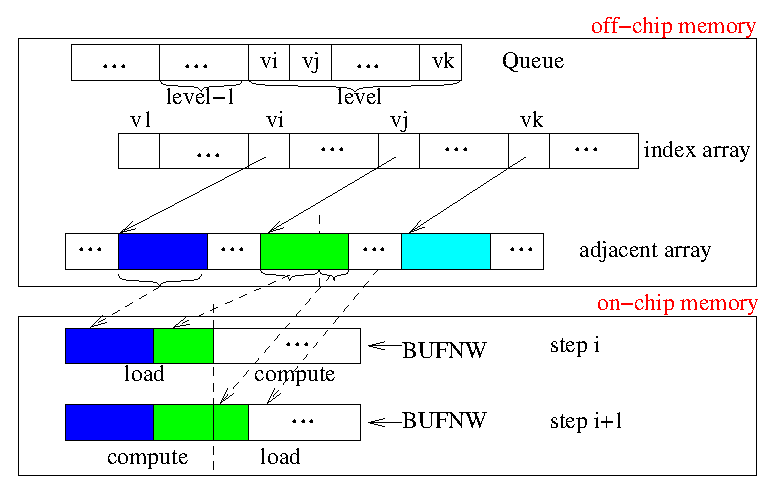
\includegraphics[width=5in,height=2.5in]{Img/Chap_Algorithm/db}
		\caption{double-buffering中的片外和片内存储映像。}
		\label{fig:db}
	\end{center}
\end{figure}


\subsection{数据流体系结构中硬件锁同步的优化}
当线程遍历同一级中顶点的邻接点时,如果存在相同的邻接点,冲突发生,这时需要某种同步方式处理冲突情况。粗粒度锁同步对整个邻接数组分配一个全局锁,
每个线程需要获取顶点遍历其邻接点都需要先获得锁。然而,事实上,并不是每次都存在冲突,所以这种粗粒度锁效率较低。细粒度锁给每个顶点赋予一个
锁变量,显然,在常规体系结构上,需要一个和邻接数组一样大小的数组保存锁变量。在本研究中的多核体系结构中,锁数组的大小通常超过片内存储而产
生大量的片外存储的访问,这导致性能显著下降。IBM Cyclops64处理器提供了硬件支持的细粒度锁同步机制-Synchronization State Buffer(SSB)\citep{ssb-isca07}。和
Cray MTA-2中的full/empty存储位机制不同,SSB在存储控制中增加了一个小的额外存储,记录和管理正在使用的锁同步的数据单元的状态。当某个存储地
址需要一个线程单独访问,SSB分配一个空间纪录该存储位置,而不是一开始就为可能使用的锁分配所有的空间。SSB的提出基于一个重要而合理的假设:在
任何时刻,被同步的存储位置只有很小的一部分正在被使用。也就是说,尽管在程序运行的整个生命周期,大量的锁同步需要使用,但在具
体的某个时刻,只有相当少部分的锁同步被使用。图\ref{fig:ssb-entry}是SSB中一个元素的结构。每个元素由4部分组成:1)地址域保存需要锁同步的存
储地址;2)参与同步的线程ID;3)8位的计数器;4)4位状态域支持16种不同同步操作状态。具体的SSB实现和解释请阅读参考文献。这里基于SSB实现了BFS中
的细粒度同步并行算法,算法\ref{algo:ssb}中的{\it swlock\_l} 和{\it sunlock}是对存储地址的获取锁和释放锁的函数。
\begin{figure}[!htbp]
	\begin{center}
		\includegraphics[scale=0.6]{Img/Chap_Algorithm/entry}
		\caption{SSB结构} \label{fig:ssb-entry}
	\end{center}
\end{figure}

\begin{algorithm}\label{algo:ssb}
	{\bf  BFS based on SSB on IBM Cyclops64}
	{\bf for} $w \in NW_{level}$ {\bf pardo}\\
	\hspace*{1pc}{\it rt = swlock\_l(\&(d[w]), \&dd);}\\
	\hspace*{1pc}{\bf if} rt == 0\\
	\hspace*{2pc}{\bf if} $d[w]<0$ {\bf then}\\
	\hspace*{3pc}enqueue $w\rightarrow Q_{level+1}$\\
	\hspace*{3pc}$d[w]\leftarrow d[v]+1$\\
	\hspace*{3pc}$\sigma[w]\leftarrow \sigma[w]+\sigma[v]$\\
	\hspace*{3pc}append $v\rightarrow P[w]$\\
	\hspace*{2pc}{\bf else if} $d[w]=d[v]+1$ {\bf then}\\
	\hspace*{3pc}$\sigma[w]\leftarrow \sigma[w]+\sigma[v]$\\
	\hspace*{3pc}append $v\rightarrow P[w]$\\
	\hspace*{2pc}{\it sunlock(\&(d[w]));}\\
	\hspace*{1pc}{\bf else if} $d[w]=d[v]+1$ {\bf then}\\
	\hspace*{2pc}{\bf while} ((rt = {\it swlock\_l(\&(d[w]), \&dd))} != 0);\\
	\hspace*{2pc}$\sigma[w]\leftarrow \sigma[w]+\sigma[v]$\\
	\hspace*{2pc}append $v\rightarrow P[w]$\\
	\hspace*{2pc}{\it sunlock(\&(d[w]));}
\end{algorithm}

评价图算法
性能的主要指标使用Bader等提出用于评价HPCS高性能计算机系统的基准测试程序SSCA2中的TEPS(traversed edges per
second)。假设顶点个数是$n=2^{scale}$,边数是$E(n)$\footnote{有时候为了简化问题规模,图遍历时只选择权值能被8整除的边},程序的运行时间用$T(n)$表示,TEPS定义
为平均每秒访问的边数$TEPS(n)=\frac{n*E(n)}{T(n)}$。实验测试了并行算法的弱可扩展性和强可扩展性。在传统的高性能计算机系统上,如果并行程序能够
获得高的弱可扩展性即可,即主要追求通过同时增加处理器和问题规模获得加速。在大规模多核体系结构中,处理核的数量正逐渐增加,但每个核的处理速度却呈
下降趋势,主要通过增加并行性来提高程序性能。因此,更合理的评价是在固定问题规模而只增加核的数目条件下测试并行程序的加速比。这意味者强可扩展性
应称为大规模多核上细粒度并行算法的更重要评价参数。事实上,这种要求也有利于在大多数情况下只能运行小规模程序的模拟器上开发和评价算法。
\begin{figure}[htbp]
	\begin{center}
		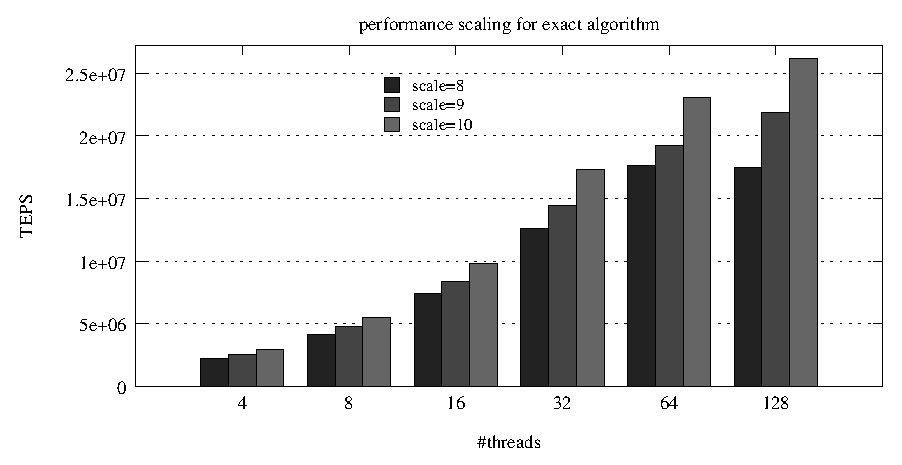
\includegraphics[scale=0.6]{Img/Chap_Algorithm/teps}
		\caption{并行介度中心算法的TEPS性能} \label{fig:teps}
	\end{center}
\end{figure}

图\ref{fig:teps}
是并行程序的TEPS性能。和SSCA2中的简单细粒度并行算法相比较,优化后的细粒度并行算法大大减低了运行时间而且
显示了随线程规模良好的可扩展性。尽管问题规模相当小,优化的细粒度并行算法仍然在线程数小于32时取得了线性加速比。在测试的最小问题规模为$scale=8$中,
当线程个数超过128时没有明显的性能提高,但在更大的问题规模$scale=9,10$时,算法也能取得加速比。注意到并行算法的中粒度和细粒度并行性的获得都和顶点
的度数有关。$scale=8$的情况下,图中的顶点的最大度只有64,因此存在的并行性导致在128个线程时不能获得好的性能; $scale = 9,
10$时,最大度分别是94和348,算法依然能够获得一定的扩展性能。


\section{科学计算-高性能稠密矩阵算法}\label{sec:PM_mm}
本节基于一种流行的细粒度多线程众核结构GPU上验证渗透算法设计模型的对稠密矩阵乘算法优化的有效性。首先介绍稠密矩阵乘算法基本概念和在众核上性能优化存在的问题。然后,描述在CUDA体系结构和编程模型中,基于渗透模型的稠密矩阵乘的流水线算法设计。进一步,基于NVIDIA GPU的体系结构(Fermi)提出一种更好隐藏长延迟指令的优化流水线的指令调度算法。

\subsection{稠密矩阵乘算法介绍}
稠密矩阵运算是科学计算和工程计算中的重要问题,是基础线性代数子程序(BLAS)库重要的一个核心算法。该规范定义DGEMM为 C := alpha * A * B + beta * C,其中A,B和C分别是m * k, k * n, m * n的矩阵。DGEMM的一个简单实现是三层循环嵌套。由于分块矩阵-矩阵乘法实现了更多的数据复用和更高的有效内存帶宽,分块矩阵乘法算法在具有内存层次结构的处理器上会有更高的性能。

大量的研究工作指出,全局内存的延迟和帶宽对DGEMM的效率有重要影响。对GPU上的分块DGEMM算法,A,B,C三个矩阵分别被分成bm*bk,bk*bn,bm*bn大小的块,这些块分别分布成M*K,K*N,M*N的网格,其中M=m/bm, N=n/bn, K=k/bk。计算是在一个二维的线程块网格上完成的,每一C的子块分配给一个线程块。也就是说,共有M*N个线程块,每个线程块都需要分别获取K个A和B的子块。这些内存读从全局内存读取了M*N*K*bm*bk+M*N*K*bk*bn=m*n*k*(1/bm+1/bn)个双精度浮点数。分块算法让全局内存帶宽需求减少了2/(1/bm + 1/bn)倍。此外,由于A和B的块都是首先加载到共享内存中,数据将被重用多次,从而减少了全局内存访问的代价。

GPU上的内存层次结构抽象为三个层次:片外内存(全局内存),片上内存(cache或者共享内存)和寄存器文件。从全局内存层次到寄存器层次,相邻层之间的帶宽增加且延迟减少。因此,分块算法通常包含两层分块。对于我们分块DGEMM算法而言,我们将从全局内存到共享内存层次的分块称为共享内存分块。由于共享内存和寄存器文件之间存在带宽和延迟的差距,共享内存中的子矩阵的分块对于重用寄存器中的数据是必要的。我们将这一层分块称为寄存器分块。此外,为了最大限度地提高浮点执行单元的效率,共享内存和寄存器文件的利用是另一个关键因素。举例来说,共享内存中的数据布局和访问模式应该仔细安排以避免bank冲突,这些冲突会导致额外的访存延迟。每个线程使用的寄存器数量也应该平衡以保持足够的线程并发来掩盖延迟。

算法\ref{algo:dgemmV0}是具有全局内存和共享内存层次的两层分块算法。矩阵A在进行矩阵乘之前转置了。本文中的实验结果包含了转置的开销,占了大约1\%的算法执行时间。在伪代码中还有几个未定义的参数(如bm,bn…),这些参数对性能有直接影响。
\begin{figure}[htbp]
	\begin{center}
		\includegraphics[scale=0.8]{Img/Chap_Algorithm/dgemmV0}
		\caption{DGEMM例程基础算法} \label{fig:dgemmV0}
	\end{center}
\end{figure}

\subsection{渗透模型的流水算法设计}
对算法模型的深度分析表明采用更宽的如128位内存操作可提高获得更高的浮点性能的空间\citep{},但需要新的线程-数据映射策略。两个warp加载长度为64(bm或bn)的A/B的一列/一行,每个线程加载一个64位的双精度数据。如果使用128位的内存指令,我们只需要32个线程(1个warp),每个线程加载两个双精度数据(128位)。因此我们将线程块由64*4改为32*8。图7描述了两种不同内存指令模式下数据-线程的映射情况。其中左边的图展示了使用64位内存取数指令将64*16的数据块从全局内存读取到共享内存中的过程,右边的图展示了使用128位内存取数指令的情况。

\begin{figure}[htbp]
	\begin{center}
		\includegraphics[scale=0.8]{Img/Chap_Algorithm/DGEMMpipeline}
		\caption{全局内存和共享内存间数据传输的数据线程映射。这张图由虚线分为两部分。左边阐明了算法2使用64位内存指令的映射。右边阐明了算法3使用128位内存指令的映射。} \label{fig:DGEMMpipeline}
	\end{center}
\end{figure}

假设矩阵以列向布局存储在全局内存中,而块以行向布局存储在共享内存中。如图~\ref{fig:DGEMMpipeline}所示,对大小为64*16的的块,使用64位内存指令时每个线程需要发射4条存取指令,而128位模式下每个线程只需要发射2条存取指令。例如,发射4条64位内存指令时,线程0…63取0,4,8,12列(图中蓝色的列),线程64…127取1,5,9,13列(图中黑红色的列),线程128…191取列2,6,10,14列(图中红色的列),线程192…255取3,7,11,15列(图中黄色的列)。在共享内存中,64个双精度数(64位)的一列存储为一行,然后由一列64个线程连续访问。图~\ref{fig:DGEMMpipeline}中右图阐明了128位内存操作模式下相应的数据-线程映射。线程0…31取0,8列(图中蓝色的列),线程32…63取1,9列(图中黑红色的列)。类似地,每一列线程通过2条128位内存指令取2列(同样颜色的列)

如果我们把Fermi的存储层次抽象为由全局内存和共享内存组成的两层,Fermi与其它带有显示的软件控制内存架构的众核架构如IBM Cell和IBM Cyclops64处理器非常类似。经验表明,在低延迟的内存中使用双缓冲的软件流水是一种有效的把计算和跨内存层次的通信重叠的方法。
为了实现一个双缓冲策略,我们将大小为64*16的块分为两块64*8大小的块。当前半部分用于计算矩阵C时,取后半部分数据的指令也会发射。线程调度程序负责将计算与内存操作重叠。双缓冲算法如图8所示。在伪代码中,我们将smA/B[0…bk/2-1][bm]映射为图7中的缓冲区0,smA/B[bk/2-1…bk-1][bm]映射为缓冲区1。在while循环中,指令被同步操作分组为内存和计算指令。由于它们操作不同的共享内存缓冲区,内存操作与计算可以并行进行。这些指令间没有数据依赖,因此还有空间通过指令调度优化来隐藏内存延迟。

新算法没有使用额外的寄存器实现双缓冲策略。事实上,一个重要的变化是使用了高延迟的128位内存指令。此外,为了确保下一块数据在计算之前完全被加载到共享内存中,双缓冲策略迫使我们在while循环中使用另一条同步指令。显然,除了128位内存指令的高延迟,额外的同步也带带来额外的延迟。由于双缓冲算法的主要代价是额外延迟,因此我们认为这里有通过指令调度来隐藏这些延迟的空间。
\begin{figure}[htbp]
	\begin{center}
		\includegraphics[scale=0.8]{Img/Chap_Algorithm/DGEMMPipeAlgo}
		\caption{双缓冲策略优化后的算法。} \label{fig:DGEMMPipeAlgo}
	\end{center}
\end{figure}


\subsection{体系结构相关的优化实现}
算法3中的while循环占用了大部分执行时间。我们的指令调度主要关注这段代码。在详细介绍指令调度的算法之前,我们首先计算出执行这段代码的指令组合比例。表3总结了指令组合的比例。如前所述,每个线程从全局内存加载一个元素(4字,在下文中,我们用一个元素指代128位的数据)到共享内存中两个缓冲中的一个(参看算法3中的6-7,14-15行)。由于没有内存到内存的指令,一次数据移动操作被转换为两条内存指令:一条加载指令(ld.gm.128)将数据从全局内存加载到寄存器,一条存储指令(st.sm.128)将数据从寄存器存储到共享内存中。每个while循环将发射4条指令来填充双缓冲区。现在让我们检查每个半缓冲区的两个内部循环。在每个ki循环中,每个线程将A的两个元素和B的两个元素读入寄存器,然后计算C的一个4*4的字块。内存操作有4条共享内存的加载指令(ld.sm.128)组成,计算操作由16条浮点指令(dfma)组成。对bk=16来说,总共有64条ld.sm.128和256条dfma指令。此外,我们需要10条整数指令和一条分支指令来进行地址计算和循环控制。

为了方便调度指令执行顺序,我们测量了while循环中使用的指令的流水线延迟。表3列出了指令延迟。由于数据依赖性,我们将延迟分为两种类型:写后读(RAW)和读后写(WAR)。例如,假设指令y依赖于指令x,写后读延迟就是从指令x发射到读取指令x写入寄存器的值的y指令可以发射这中间经历的时钟周期数。读后写延迟是从指令x发射到写入指令x读取寄存器的y指令可以发射这中间经历的时钟周期数。

\begin{figure}[htbp]
	\begin{center}
		\includegraphics[scale=0.8]{Img/Chap_Algorithm/InstrSched}
		\caption{内存循环指令调度算法。} \label{fig:InstrSched}
	\end{center}
\end{figure}

指令流的执行是根据测量到的延迟来调度的。给定一个指令序列,我们扫描代码,对于每条指令,我们计算该指令使寄存器的值可用需要多长时间。例如ld.gm.128 r2,[r1]指令,寄存器r2,r3,r4,r5的值在指令发出几百个循环后才可用。在我们的调度算法中,我们将这种延迟称为寄存器的有效时间(即r2的有效时间为332∼1000个周期,这取决于数据是否缓存)。我们动态地构造了两个map表last\_raw和last\_war来记录每条指令的寄存器名及其有效时间(如last\_raw[r2] = 1000)。与此同时,我们跟踪直到当前指令发射的累计执行时间(tcurr)。我们会检测当前指令需要的寄存器是否处于last\_raw或last\_war表中。如果这些寄存器不在这两张表中,则由于没有数据依赖它的发射阻塞时间为0。否则,如果其中一个寄存器出现在两张表中的任意一张,则当前指令发射的阻塞时间由寄存器的有效时间和当前时间只差计算得到。例如,如果在指令 ld.gm.128 r2,[r1]扫描之后指令 st.sm [smA],r2,则它的发射阻塞时间为last\_raw[r2] - tcurr。假设ld.gm指令和st.sm指令之间有4条独立指令,这四条独立指令每条都有6个时钟周期的无阻塞发射到发射延迟,则观察到的ld.gm到st.sm之间的延迟(或者说st.sm额外阻塞的时间)是1000-(t\_curr=4*6+6)=970个时钟周期(st.sm有6个时钟周期的延迟)。指令调度的目标是使所有指令的累计延迟时间最小。


首先,我们重新排列每个内部for循环的指令序列。图~\ref{fig:InstrSched}展示了内部for循环中的前两个循环的指令重新排序示例。每个循环有4条ld.sm.128指令后面跟着16条 dfma指令。表面上看执行顺序不能改变因为寄存器rA[0…3]与寄存器rB[0…3]之间存在数据依赖。然后,如图~\ref{fig:InstrSched}所示,寄存器rA[0],rA[1]在前8条dfma指令执行后就释放了,寄存器rB[0], rB[1]在前12条dfma指令执行完之后就被释放了。这一观察结果表明,在展开的循环中插入这些加载指令以最小化阻塞时间是可行的,因为最多只用搜索8个可能得插入点。然后,我们添加了4条load/store指令的调度,这些指令将数据从全局内存加载到共享内存。由于这些指令与其它受同步限制的160条指令之间没有数据依赖关系,因此我们可以为这四条指令在这160条指令之间穷举搜索最好的插入点。最后,在两条st.sm.128指令中的第二条被调度后,我们我们从这条指令的插入点之后搜索同步指令的插入点。


\begin{figure}[htbp]
	\begin{center}
		\includegraphics[scale=0.8]{Img/Chap_Algorithm/DGEMMPerf}
		\caption{优化的DGEMM与NVIDIA CUBLAS的性能比较。} \label{fig:DGEMMPerf}
	\end{center}
\end{figure}

图~\ref{fig:DGEMMPerf}报告了它们的总体性能改进。它描绘了我们最终版本DGEMM函数的性能。与CUDA3.2相比,它提高了20\%的浮点性能,并达到峰值362gflops /s(浮点效率为70\%)。虽然我们的优化策略的组合确实提高了性能,但是成功的一个主要前提是我们必须手工用汇编代码来实现优化的程序。事实上,我们之前的分析表明,在选择最优的分块算法之后,DGEMM程序的性能瓶颈是延迟。特别地,128位内存指令的使用让这个问题变得更糟糕。然而,我们的优化策略减轻了指令延迟的影响,提高了性能。

\section{相关工作}

\section{总结与评述}

\section{文献索引和笔记}

\end{flushleft}